% (c) 2012 Claudio Carboncini - claudio.carboncini@gmail.com
% (c) 2012-2013 Dimitrios Vrettos - d.vrettos@gmail.com
% (c) 2015 Daniele Zambelli daniele.zambelli@gmail.com

\input{\folder divisibilita_scomposizione_grafici}

\chapter{Divisibilità e scomposizione di polinomi}

\section{Divisione tra polinomi}

\subsection{Algoritmo di Euclide}
\label{subsec:divpol_divisione_euclide}

Ricordiamo la divisione tra due numeri, per esempio~\(147:4\). Si tratta di 
trovare un quoziente~\(q\) e un resto~\(r<4\), 
in modo che~\(147=q\times~4+r\). 
Un algoritmo per trovare questi due numeri è il seguente:
\begin{center}
% \input{\folder lbr/fig001_div.pgf}\\
\divisionenumerica
\end{center}
Verifichiamo che~\(147=36\times~4+3\), dunque~\(q=36\) e~\(r=3\) soddisfano 
la nostra richiesta.

In questo paragrafo ci proponiamo di estendere questo algoritmo dal calcolo 
numerico al calcolo letterale, in particolare alla divisione tra polinomi.

Nell'insieme dei polinomi in una sola variabile, ad esempio~\(x\), vogliamo 
definire l'operazione di divisione, cioè, assegnati due polinomi, 
\(A(x)\) \emph{dividendo} e~\(B(x)\) \emph{divisore}, vogliamo determinare 
altri due polinomi, \(Q(x)\) \emph{quoziente} e~\(R(x)\) \emph{resto},
con grado di~\(R(x)\) minore del grado di~\(B(x)\), per i 
quali:~\(A(x) = B(x){\cdot}Q(x) + R(x)\).

Per eseguire l'operazione si usa un algoritmo molto simile a quello 
usato per la divisione tra numeri interi. Illustriamo l'algoritmo con 
un esempio.

% \begin{exrig}
 \begin{esempio}
Eseguire la divisione tra i polinomi~\(A(x)=3x^4+5x-4x^3-1\) 
e~\(B(x)=3x^2-1\).

Prima di eseguire l'algoritmo dobbiamo sempre controllare che:
\begin{itemize*}
 \item i polinomi siano ordinati secondo le potenze decrescenti della 
 variabile, in questo caso la~\(x\) poiché ciò
    non è vero, riscriviamo~\(A(x)\) ordinato:~\(A(x)=3x^4-4x^3+5x-1\)
 \item dividendo e divisore siano in forma completa, cioè abbiano i termini 
 con tutti i gradi; nel nostro esempio, i due polinomi non sono in
    forma completa, quindi inseriamo i termini mancanti ponendo~0 come 
    coefficiente delle potenze mancanti:
    \[A(x)=3x^4-4x^3+0x^2+5x-1; \quad B(x)=3x^2+0x-1\]
\end{itemize*}

% \newpage %-----------------------------------------

% I passi da eseguire sono i seguenti:
\begin{comment}

\affiancati{\primo}{\secondo}{
}{
}

\end{comment}
\def \primo{.39}
\def \secondo{.59}

\begin{enumerate*}
 \item 
\affiancati{\primo}{\secondo}{
 Disponiamo i polinomi secondo il seguente schema, del tutto simile a 
 quello usato per la divisione tra numeri.
}{
\begin{center} \divpola \end{center}
}
 \item 
\affiancati{\primo}{\secondo}{
 Dividiamo il primo termine del dividendo per il primo termine del divisore, 
 otteniamo~\(x^2\) che è il primo termine del quoziente;
 esso va riportato nello spazio dedicato al quoziente.
}{
\begin{center} \divpolb \end{center}
}
 \item 
\affiancati{\primo}{\secondo}{Moltiplichiamo il primo termine ottenuto 
per tutti i termini del divisore e 
trascriviamo il risultato del prodotto sotto il dividendo,
avendo cura, per essere facilitati nel calcolo, di:
\begin{itemize*}
\item incolonnare i termini con lo stesso grado, ossia scrivere i risultati 
del prodotto in ordine da sinistra verso destra;
\item cambiare tutti i segni ottenuti, in questo modo risulta più pratico 
eseguire la somma algebrica dei polinomi invece della sottrazione.\\
\end{itemize*}
}{
\begin{center} \divpolc \end{center}
}
 \item 
\affiancati{\primo}{\secondo}{
Sommiamo il dividendo con il polinomio sottostante e riportiamo il risultato 
in un'altra riga. Questo polinomio si chiama primo resto parziale.
Notiamo che ha grado~\(3\), maggiore del grado~\(2\) del divisore, pertanto 
la  divisione va continuata.\\
}{
\begin{center} \divpold \end{center}
}
 \item 
\affiancati{\primo}{\secondo}{
Ripetiamo il procedimento tra il resto parziale ottenuto, 
\(-4x^3+x^2+5x-1\) e il divisore~\(3x^2+0x-1\). Dividiamo il primo 
termine  del resto che è~\(-4x^3\) per il primo termine del divisore che 
è~\(3x^2\). 
Otteniamo~\(-{\dfrac{4}{3}}x\) che è il secondo termine del quoziente.
}{
\begin{center} \divpole \end{center}
}
 \item 
\affiancati{\primo}{\secondo}{
Proseguiamo moltiplicando~\(-{\dfrac{4}{3}}x\) per~\(B(x)\), riportiamo il 
risultato del prodotto, con segno opposto, sotto i
termini del primo resto parziale e addizioniamo i due polinomi.
}{
\begin{center} \divpolf \end{center}
}
 \item 
\affiancati{\primo}{\secondo}{
Possiamo ripetere per l'ultima volta il procedimento precedente tra il 
resto parziale~\(R_{p}(x)=x^2+\dfrac{11}{3}x-1\) e
il divisore~\(B(x)\) in quanto hanno lo stesso grado. Dividendo il 
termine di grado maggiore di~\(R_{p}(x)\), che è~\(x^2\),
per il termine di grado maggiore di~\(B(x)\) che è~\(3x^2\) si 
ottiene~\(\dfrac{1}{3}\) che è il terzo termine del polinomio quoziente.
}{
\begin{center} \divpolg \end{center}
}
\end{enumerate*}

Non possiamo più ripetere l'algoritmo poiché il resto ottenuto ha grado 
minore del grado del divisore.

In conclusione~\(A(x):B(x)\) ha 
quoziente~\(Q(x)=x^2-\dfrac{4}{3}x+\dfrac{1}{3}\) e 
resto~\(R(x)=+{\dfrac{11}{3}}x-\dfrac{2}{3}\).

\paragraph{Verifica}
Verifichiamo se abbiamo svolto correttamente i calcoli; dovrebbe risultare, 
come detto sopra:\(Q(x)\cdot B(x)+R(x) = A(x)\).
\begin{equation*}
\begin{split}
Q(x)\cdot B(x)+R(x) &= 
\tonda{3x^2-1}\tonda{x^2-\dfrac{4}{3}x+\dfrac{1}{3}}+
\dfrac{11}{3}x-\dfrac{2}{3} =\\ 
&=3x^4-4x^3+x^2-x^2+\dfrac{4}{3}x-
  \dfrac{1}{3}+\dfrac{11}{3}x-\dfrac{2}{3}=\\
&= 3x^4-4x^3+\dfrac{15}{3}x-\dfrac{3}{3}
= 3x^4-4x^3+5x-1 = A(x).
\end{split}
\end{equation*}
I polinomi~\(Q(x)\) e~\(R(x)\) soddisfano quindi le nostre richieste. 
Ma sono unici? È sempre possibile trovarli? 
A queste domande risponde il seguente teorema.
 \end{esempio}
% \end{exrig}

\begin{teorema}[Divisione euclidea]
 Siano~\(A(x)\) e~\(B(x)\) due polinomi in una sola variabile, esistono 
 e sono  unici due polinomi~\(Q(x)\) e~\(R(x)\), con grado di~\(R(x)\)
 minore o uguale del grado di~\(B(x)\), 
 tali che~\(A(x)=Q(x)\cdot B(x)+R(x)\).
\end{teorema}

\osservazione Nel caso in cui il grado di~\(A(x)\) sia minore del grado 
di~\(B(x)\) il teorema resta valido, 
in questo caso~\(Q(x)=0\) e~\(R(x)=A(x)\).
Nel caso di polinomi in più variabili il teorema della divisione 
euclidea non vale.

\begin{definizione}
 Si dice che un polinomio~\(A\) (dividendo) è divisibile per un 
 polinomio~\(B\)  (divisore) se esiste un polinomio~\(Q\) (quoziente) 
 per il quale~\(A=Q \cdot B\).
\end{definizione}

% \begin{exrig}
 \begin{esempio}
 Eseguiamo la divisione tra~\(A(x)=x^3-2x^2+x-2\) e~\(B(x)=x^2+1\).
I due polinomi sono ordinati secondo potenze decrescenti della variabile, 
il grado di~\(A\) è maggiore del grado di~\(B\) e quest'ultimo
deve essere completato. 
Eseguendo la divisione: 
\begin{center}
% \input{\folder lbr/fig009_div.pgf}\vspace*{-1.10ex}
\divdue
\end{center}
 \end{esempio}
\noindent otteniamo:
\(\tonda{x^3-2x^2+x-2}:\tonda{x^2+1}=(x-2)\) 
il resto~\(R(x)\) è il polinomio nullo e~\(A(x)\) è divisibile per~\(B(x)\).
Infatti~\(\tonda{x^2+1}\cdot (x-2)=\tonda{x^3-2x^2+x-2}\).
% \end{exrig}

In conclusione, se~\(A(x)\) è un polinomio di grado~\(n\) e~\(B(x)\) un 
polinomio di grado~\(m\) con~\(n\ge m\), quando si esegue la divisione 
tra~\(A\) e~\(B\) si ottiene un polinomio quoziente~\(Q(x)\) 
di grado~\(n-m\) e un polinomio~\(R(x)\) di grado~\(g<m\).
Si dimostra che i polinomi~\(Q(x)\) e~\(R(x)\) sono unici.

Se~\(R(x)\) è il polinomio nullo, la divisione è esatta e il polinomio~\(A\) 
è divisibile per il polinomio~\(B\).

% \vspazio\ovalbox{\risolvii \ref{ese:12.1}, \ref{ese:12.2}, \ref{ese:12.3}, 
% \ref{ese:12.4}, \ref{ese:12.5}}

% \section{Polinomi in più variabili}
% Per la divisione tra polinomi in più variabili riportiamo soltanto qualche 
% esempio
% % \begin{exrig}
%  \begin{esempio}
% Siano~\(A(a,b)=3a^{2}b+4ab^{2}+3a^{3}-2b^{3}\) e~\(B(a,b)=a-3b\) 
% rispettivamente 
% dividendo e divisore di una divisione tra polinomi;
% essi sono due polinomi omogenei nelle due variabili~\(a\) e~\(b\) 
% rispettivamente 
% di grado~\(3\) e grado~\(1\).
% 
% Per eseguire la divisione procediamo come nel caso di polinomi in una sola 
% variabile.
% Dividiamo il polinomio~\(A(a,b)=3a^{2}b+4ab^{2}+3a^{3}-2b^{3}\) per il 
% polinomio~\(B(a,b)=a-3b\) rispetto alla variabile~\(a\).
% Controlliamo le condizioni:
% \begin{itemize*}
% \item \(A\) e~\(B\) sono ordinati rispetto alla variabile a? No. \(A\) non 
% lo è. 
% Quindi ordiniamo~\(A\):
% \[A(a,b)=3a^{3}+3a^{2}b+4ab^{2}-2b^{3};\]
% \item il grado di~\(A\) è maggiore o uguale al grado di~\(B\)? Sì;
% \item \(A\) e~\(B\) sono completi rispetto alla variabile~\(a\)? Sì.
% \end{itemize*}
% Costruiamo lo schema per eseguire l'algoritmo e procediamo:
% \begin{center}
%  \input{\folder lbr/fig011_eser.pgf}
% \esedivisioneb
% \end{center}
% Il quoziente è~\(Q =\ldots \ldots \ldots\) il resto~\(R = 118b^{3}\)
% 
% Verifica~\(\ldots \ldots \ldots \ldots \ldots \ldots\)
% 
% Se avessimo eseguito la divisione rispetto alla variabile~\(b\), avremmo 
% ottenuto stesso quoziente e stesso resto? Proviamo.
% Controlliamo le condizioni:
% \begin{itemize*}
% \item \(A\) e~\(B\) sono ordinati rispetto alla variabile~\(b\)? No. 
% Ordinando~\(A\), 
% risulta:
% \[A(a,b)=-2b^{3}+4ab^{2}+3a^{2}b+3a^{3}+3a^{2}b;\]
% e ordinando~\(B\), risulta
% \[B(a,b)=-3b+a;\]
% \item il grado di~\(A\) è maggiore o uguale al grado di~\(B\)? Sì;
% \item \(A\) e~\(B\) sono completi rispetto alla variabile~\(b\)? Sì.
% \end{itemize*}
% Costruisci lo schema dell'algoritmo e concludi.
%  \end{esempio}
% % \end{exrig}
% \ovalbox{\risolvii \ref{ese:12.6}, \ref{ese:12.7}}

\subsection{Regola di Ruffini}
\label{subsec:divpol_divisione_ruffini}

Per eseguire la divisione tra due polinomi, \emph{nel caso in cui il
divisore sia del tipo \((x+a)\)} si può applicare la regola di Ruffini.
Questa regola deriva dall'algoritmo di Euclide ma lo rende più semplice.

% \begin{procedura}
%  Dividere un polinomio con la regola di Ruffini:
% 
%  \begin{enumeratea}
%  \item calcolo del resto;
% \item applicazione del procedimento di divisione;
% \item verifica.
%  \end{enumeratea}
% \end{procedura}

Partiamo da un esempio e eseguiamo innanzitutto la divisione con l'algoritmo 
di Euclide:

% ( 3 x^4 +8 x^3 +9 x^2 +4 x -5 ) : ( x +2 ) = 3 x^3 +2 x^2 +5 x -6, R= 7 %

\[\tonda{3 x^4 +8 x^3 +9 x^2 +4 x -5} : (x + 2)\]

Utilizzando l'algoritmo di Euclide otteniamo:

\begin{inaccessibleblock}[Algoritmo euclideo della divisione per i polinomi]
% \vspace{-2ex}
\begin{center}
% % (c) 2012 Dimitrios Vrettos - d.vrettos@gmail.com
\begin{tikzpicture}[font=\small]

\matrix  (a) [matrix of  nodes, anchor=south, minimum width=9mm,nodes={text depth=0mm}]{
$ 3x^4$ & $+8x^3$ & $+9x^2$ & $ +4x$ & $ -5$  & $ x   $ & $+2$    &  {}   &  {}  \\
$-3x^4$ & $-6x^3$ &    {}   &   {}   &   {}   & $ 3x^3$ & $+2x^2$ & $+5x$ & $ -6$\\
  {}    & $+2x^3$ & $+9x^2$ &   {}   &       \\
  {}    & $-2x^3$ & $-4x^2$ &   {}   &   {}   &   {}    &  R$=+7$\\
  {}    &   {}    & $+5x^2$ & $ +4x$ &   {}  \\
  {}    &   {}    & $-5x^2$ & $-10x$ &   {}  \\
  {}    &   {}    & $ {}  $ & $ -6x$ & $ -5$ \\
  {}    &   {}    & $ {}  $ & $ +6x$ & $+12$ \\
  {}    &   {}    & $ {}  $ & $ {} $ & $+7$ \\
};

\draw(a-1-5.north east)--(a-9-5.south east);
\draw(a-2-6.north west)--(a-2-9.north east);
\draw (a-2-1.south west) -- (a-2-3.south east);
\draw (a-4-2.south west) -- (a-4-4.south east);
\draw (a-6-3.south west) -- (a-6-5.south east);
\draw (a-8-4.south west) -- (a-8-5.south east);
%  \draw (a-4-2.south west) -- (a-4-4.south east);
\end{tikzpicture}
\ruffinia
\end{center}
% \vspace*{-1.10ex}
% \vspace{-2ex}
\end{inaccessibleblock}

Possiamo osservare che la parte letterale è facilmente ricostruibile, se 
abbiamo messo per bene in colonna, e molti coefficienti sono inutilmente 
ripetuti. Riscriviamo la divisione senza la parte letterale e con i
coefficienti essenziali riquadrati:

\begin{inaccessibleblock}[Solo i coefficienti della divisione tra polinomi.]
% \vspace{-2ex}
\begin{center}
%  % (c) 2012 Dimitrios Vrettos - d.vrettos@gmail.com
% (c) 2015 Daniele Zambelli - daniel.zambelli@gmail.com

\begin{tikzpicture}[font=\small, %minimum size=6mm,
data/.style={
rectangle,
minimum size=6mm,
top color=white,
bottom color=red!50!black!20,
% font=\small
},
interm/.style={
rectangle,
minimum size=6mm,
draw=black,
% font=\small
},
result/.style={
rectangle, rounded corners=3mm,
minimum size=6mm,
draw=black,
% font=\small
}]
% \begin{tikzpicture}[font=\small]

\matrix  (a) [matrix of  nodes, anchor=south, minimum width=9mm,
              nodes={text depth=0mm}]{
\node[result, data]{$+3$}; & \node[data]{$+8$}; & \node[data]{$+9$}; & 
\node[data]{$ +4$}; & \node[data]{$ -5$};  & {} &$ 1   $ & \node[data]{$+2$};    &  {}   &  {}  \\
$-3$ & \node[interm]{$-6$}; &  {}  &  {}   & {} &  {}   & $ 3$ & $+2$ & $+5$ & $ -6$\\
 {}    & \node[result]{$+2$}; & $+9$ &   {}   & {} & \\
 {}    & $-2$ & \node[interm]{$-4$}; &   {}   & {} &  {}   &   {}    &  R$=+7$\\
 {}    &  {}  & \node[result]{$+5$}; & $ +4$ &   {} & {} &\\
 {}    &  {}  & $-5$ & \node[interm]{$-10$}; &   {} & {} &\\
 {}    &  {}  & ${}$ & \node[result]{$ -6$}; & $ -5$ & {} &\\
 {}    &  {}  & ${}$ & $ +6$ & \node[interm]{$+12$}; & {} &\\
 {}    &  {}  & ${}$ & $ {}$ & \node[result]{$+7$}; & {} &\\
};

\draw(a-1-6.north east)--(a-9-6.south east);
\draw(a-2-7.north west)--(a-2-10.north east);
\draw (a-2-1.south west) -- (a-2-3.south east);
\draw (a-4-2.south west) -- (a-4-4.south east);
\draw (a-6-3.south west) -- (a-6-5.south east);
\draw (a-8-4.south west) -- (a-8-6.south east);
%  \draw (a-4-2.south west) -- (a-4-4.south east);
\end{tikzpicture}
\ruffinib
\end{center}
% \vspace*{-1.10ex}
% \vspace{-2ex}
\end{inaccessibleblock}

In questa versione senza le variabili sono stati evidenziati i dati,
riquadrati i risultati intermedi e cerchiati i risultati.
Tutti gli altri valori sono inutili o ripetuti. 

La regola di Ruffini permette di scrivere solo i dati necessari,
ma come si possono ottenere tutti i coefficienti senza l'algoritmo di Euclide?
Lo vediamo in questo esempio:
\affiancati{.50}{.50}{
% \begin{multicols}{2}
\begin{itemize*}
 \item \(-2\) è l'opposto del termine noto del divisore;
 \item addiziono \(+3\) con \(0\) e ottengo \(+3\);
 \item moltiplico \(-2\) con \(+3\) e ottengo \(-6\);
 \item addiziono \(+8\) con \(-6\) e ottengo \(+2\);
 \item moltiplico \(-2\) con \(+2\) e ottengo \(-4\); 
 \item addiziono \(+9\) con \(-4\) e ottengo \(+5\);
 \item moltiplico \(-2\) con \(+5\) e ottengo \(-10\); 
 \item addiziono \(+4\) con \(-10\) e ottengo \(-6\);
 \item moltiplico \(-2\) con \(-6\) e ottengo \(+12\); 
 \item addiziono \(-5\) con \(+12\) e ottengo \(+7\).
\end{itemize*}
% \end{multicols}

Come è riassunto nel diagramma a fianco dove le frecce 
verdi tratteggiate indicano \emph{addizioni} e quelle 
rosse punteggiate indicano \emph{moltiplicazione}.

}{
\vspace*{1em}
\begin{inaccessibleblock}[Divisione con il metodo di Ruffini.]
% \vspace{-2ex}
\begin{center}
% % (c) 2012 Dimitrios Vrettos - d.vrettos@gmail.com
% (c) 2015 Daniele Zambelli - daniel.zambelli@gmail.com

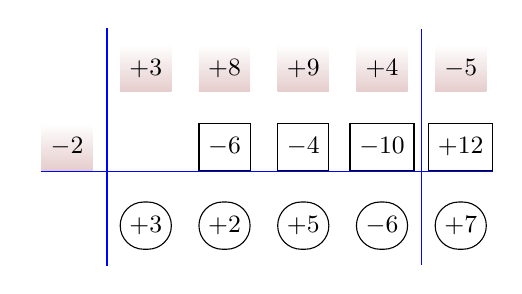
\begin{tikzpicture}[font=\small, %minimum size=6mm,
data/.style={
rectangle,
minimum size=6mm,
top color=white,
bottom color=red!50!black!20,
% font=\small
},
interm/.style={
rectangle,
minimum size=6mm,
draw=black,
% font=\small
},
result/.style={
rectangle, rounded corners=3mm,
minimum size=6mm,
draw=black,
% font=\small
},
x=10mm, y=10mm, minimum size=10mm]


% \begin{tikzpicture}[font=\small,x=8mm, y=8mm, minimum size=10mm]

\node (a0) at (0,0) {};
\node [data](a1) at (1,0) {$+3$};
\node [data](a2) at (2,0) {$+8$};
\node [data](a3) at (3,0) {$+9$};
\node [data](a4) at (4,0) {$+4$};
\node [data](a5) at (5,0) {$-5$};

\node [data](a6) at (0,-1) {$-2$};
\node (a7) at (1,-1) {};
\node [interm](a8) at (2,-1) {$-6$};
\node [interm](a9) at (3,-1) {$-4$};
\node [interm](a10) at (4,-1) {$-10$};
\node [interm](a11) at (5,-1) {+12};

\node (a12) at (0,-2) {};
\node [result](a13) at (1,-2) {$+3$};
\node [result](a14) at (2,-2) {$+2$};
\node [result](a15) at (3,-2) {$+5$};
\node [result](a16) at (4,-2) {$-6$};
\node [result](a17) at (5,-2) {$+7$};

\begin{scope}[blue]
\draw (a0.north east)--(a12.south east);
 \draw (a6.south west)--(a11.south east);
% \draw (a4.north east)--(a16.south east);
\draw (4.5, 0.5)--(4.5, -2.5);
\end{scope}

% \matrix (a)[matrix of nodes, nodes in empty cells,
%             nodes={ text width=8mm, text depth=1mm, text centered}]
% {
%  {}  & \node [data]{$+3$}; & \node [data]{$+8$}; & \node [data]{$+9$}; & \node [data]{$+4$};  & \node [data]{$-5$}; \\
% $-2$ &  {}  & $-6$ & $-4$ & $-10$ & $+12$ \\
%  {}  & $+3$ & $+2$ & $+5$ & $-6$  & $+7$  \\
% };  
% \begin{scope}[blue]
% \draw(a-1-2.north west)--(a-3-2.south west);
% \draw(a-2-1.south west)--(a-2-6.south east);
% \draw(a-1-5.north east)--(a-3-5.south east);
% \end{scope}

\end{tikzpicture}
\ruffinic
\end{center}
% \vspace*{-1.10ex}
% \vspace{-2ex}
\end{inaccessibleblock}

\vspace{1em}
\begin{inaccessibleblock}[Divisione con il metodo di Ruffini.]
% \vspace{-2ex}
\begin{center}
% % (c) 2012 Dimitrios Vrettos - d.vrettos@gmail.com
% (c) 2015 Daniele Zambelli - daniel.zambelli@gmail.com

\usepgflibrary{arrows.meta}

\begin{tikzpicture}[font=\small, x=10mm, y=10mm, minimum size=10mm]

% \begin{tikzpicture}[font=\small,x=8mm, y=8mm, minimum size=10mm]

\node (a0) at (0,0) {};
\node (a1) at (1,0) {$+3$};
\node (a2) at (2,0) {$+8$};
\node (a3) at (3,0) {$+9$};
\node (a4) at (4,0) {$+4$};
\node (a5) at (5,0) {$-5$};

\node (a6) at (0,-1) {$-2$};
\node (a7) at (1,-1) {};
\node (a8) at (2,-1) {$-6$};
\node (a9) at (3,-1) {$-4$};
\node (a10) at (4,-1) {$-10$};
\node (a11) at (5,-1) {+12};

\node (a12) at (0,-2) {};
\node (a13) at (1,-2) {$+3$};
\node (a14) at (2,-2) {$+2$};
\node (a15) at (3,-2) {$+5$};
\node (a16) at (4,-2) {$-6$};
\node (a17) at (5,-2) {$+7$};

\begin{scope}[blue]
\draw (a0.north east)--(a12.south east);
 \draw (a6.south west)--(a11.south east);
% \draw (a4.north east)--(a16.south east);
\draw (4.5, 0.5)--(4.5, -2.5);
\end{scope}

% \draw (a0.north east)--(a12.south east);
% \draw (a6.south west)--(a11.south east);
% \draw (a4.north east)--(a16.south east);

\draw [-{Stealth[length=3mm, open, round]}, 
       green, loosely dashed, line width=2pt](1.3, 0) -- (1.3, -2);
% \draw [-{Stealth[length=3mm, open, round]}, 
%       red, solid, line width=2pt] 
%       (a6.east) [xshift=-0.5cm] -- (a13.north) [yshift=-0.5cm] -- (a8.west) [xshift=+0.5cm];
\draw [-{Stealth[length=3mm, open, round]}, 
       red!50, dotted, line width=2pt] 
       (0.3, -1.2) -- (1, -1.8) -- (1.7, -1.2);
\draw [-{Stealth[length=3mm, open, round]}, 
       green, loosely dashed, line width=2pt](2.3, 0) -- (2.3, -2);
\draw [-{Stealth[length=3mm, open, round]}, 
       red!50, dotted, line width=2pt] 
       (0.3, -1.2) -- (2, -1.8) -- (2.7, -1.2);
\draw [-{Stealth[length=3mm, open, round]}, 
       green, loosely dashed, line width=2pt](3.3, 0) -- (3.3, -2);
\draw [-{Stealth[length=3mm, open, round]}, 
       red!50, dotted, line width=2pt] 
       (0.3, -1.2) -- (3, -1.8) -- (3.7, -1.2);
\draw [-{Stealth[length=3mm, open, round]}, 
       green, loosely dashed, line width=2pt](4.3, 0) -- (4.3, -2);
\draw [-{Stealth[length=3mm, open, round]}, 
       red!50, dotted, line width=2pt] 
       (0.3, -1.2) -- (4, -1.8) -- (4.7, -1.2);
\draw [-{Stealth[length=3mm, open, round]}, 
       green, loosely dashed, line width=2pt](5.3, 0) -- (5.3, -2);

\end{tikzpicture}
\ruffinid
\end{center}
% \vspace*{-1.10ex}
% \vspace{-2ex}
\end{inaccessibleblock}

}
% \begin{itemize*}
%  \item \(-2\) è l'opposto del termine noto del divisore:
%  \item \(+3\) è il primo coefficiente del dividendo
%  \item \(-6 = -2 \cdot 3\) 
%  \item \(+2 = +8 -6\) 
%  \item \(-4 = -2 \cdot 2\) 
%  \item \(+5 = +9 -4\) 
%  \item \(-10 = -2 \cdot 5\) 
%  \item \(-6 = +4 -10\) 
%  \item \(+12 = -2 \cdot (-6)\) 
%  \item \(+7 = (-5)+(+12)\) 
% \end{itemize*}

E, aggiungendo le variabili, si ottiene il risultato:
\[Q = 3 x^3 +2 x^2 +5 x -6 \quad R = +7\]
come avevamo calcolato con l'algoritmo di Euclide.

Da notare che:
\begin{itemize} [nosep]
 \item la prima riga contiene i coefficienti del dividendo;
 \item il termine noto del dividendo è posto a destra della seconda 
  linea verticale;
 \item nella seconda riga, prima della prima linea verticale si scrive 
  il   termine noto del divisore cambiato di segno, così invece di 
  ricordarsi di cambiare di segno ogni volta 
  (come nell'algoritmo di Euclide), lo si fa una volta per tutte;
 \item l'algoritmo inizia con un'addizione tra il primo coefficiente del 
  dividendo e \(0\) (addizione facile);
 \item nella terza riga otteniamo i coefficienti del risultato;
 \item dividendo un polinomio di grado \(n\) per un polinomio di primo 
  grado   si ottiene un polinomio di grado \(n-1\), quindi, in questo 
  caso, il primo monomio sarà di grado \(3\);
 \item il termine in basso a destra è il resto della divisione, 
  per forza di   grado zero;
 \item se il resto della divisione è zero vuol dire che il 
  \emph{dividendo} è un multiplo del \emph{divisore}.
\end{itemize}


%
% \hfill []
% \begin{exrig}
 \begin{esempio}
Eseguire la seguente divisione:

\(\tonda{-5x^4 +50x^3 -7x +77  } : \tonda{x -10}\)
% \(\tonda{-3a+a^{3}+1}:(a-3)\)

Il divisore è del tipo \((x + x_0)\) quindi posso usare la regola di Ruffini.
Prima di tutto mettiamo in ordine il dividendo completandolo:

\(\tonda{-5x^4 +50x^3 +0x^2 -7x +77  } : \tonda{x -10}\)
% \(\tonda{-3a+a^{3}+0a^2-3a+1}:(a-3)\)

Poi inseriamo i dati nello schema di Ruffini ed eseguiamo addizioni e 
moltiplicazioni. Dobbiamo ricordarci di cambiare segno al termine noto del 
divisore

\begin{inaccessibleblock}[Divisione con il metodo di Ruffini.]
% \vspace{-2ex}
\begin{center}
% % (c) 2012 Dimitrios Vrettos - d.vrettos@gmail.com
% (c) 2015 Daniele Zambelli - daniel.zambelli@gmail.com

\begin{tikzpicture}[font=\small, %minimum size=6mm,
data/.style={
rectangle,
minimum size=6mm,
top color=white,
bottom color=red!50!black!20,
% font=\small
},
interm/.style={
rectangle,
minimum size=6mm,
draw=black,
% font=\small
},
result/.style={
rectangle, rounded corners=3mm,
minimum size=6mm,
draw=black,
% font=\small
},
x=10mm, y=10mm, minimum size=10mm]


% \begin{tikzpicture}[font=\small,x=8mm, y=8mm, minimum size=10mm]

\node (a0) at (0,0) {};
\node [data](a1) at (1,0) {};
\node [data](a2) at (2,0) {};
\node [data](a3) at (3,0) {};
\node [data](a4) at (4,0) {};
\node [data](a5) at (5,0) {};

\node [data](a6) at (0,-1) {};
\node (a7) at (1,-1) {};
\node [interm](a8) at (2,-1) {};
\node [interm](a9) at (3,-1) {};
\node [interm](a10) at (4,-1) {};
\node [interm](a11) at (5,-1) {};

\node (a12) at (0,-2) {};
\node [result](a13) at (1,-2) {};
\node [result](a14) at (2,-2) {};
\node [result](a15) at (3,-2) {};
\node [result](a16) at (4,-2) {};
\node [result](a17) at (5,-2) {};

% \draw (a0.north east)--(a12.south east);
%  \draw (a6.south west)--(a11.south east);
% \draw (a4.north east)--(a16.south east);

\begin{scope}[blue]
\draw (a0.north east)--(a12.south east);
 \draw (a6.south west)--(a11.south east);
% \draw (a4.north east)--(a16.south east);
\draw (4.5, 0.5)--(4.5, -2.5);
\end{scope}

\draw [-{Stealth[length=3mm, open, round]}, 
       green, loosely dashed, line width=2pt](1.4, 0) -- (1.4, -2);
\draw [-{Stealth[length=3mm, open, round]}, 
       red!50, dotted, line width=2pt] 
       (0.3, -1.2) -- (1, -1.8) -- (1.7, -1.2);
\draw [-{Stealth[length=3mm, open, round]}, 
       green, loosely dashed, line width=2pt](2.4, 0) -- (2.4, -2);
\draw [-{Stealth[length=3mm, open, round]}, 
       red!50, dotted, line width=2pt] 
       (0.3, -1.2) -- (2, -1.8) -- (2.7, -1.2);
\draw [-{Stealth[length=3mm, open, round]}, 
       green, loosely dashed, line width=2pt](3.4, 0) -- (3.4, -2);
\draw [-{Stealth[length=3mm, open, round]}, 
       red!50, dotted, line width=2pt] 
       (0.3, -1.2) -- (3, -1.8) -- (3.7, -1.2);
\draw [-{Stealth[length=3mm, open, round]}, 
       green, loosely dashed, line width=2pt](4.4, 0) -- (4.4, -2);
\draw [-{Stealth[length=3mm, open, round]}, 
       red!50, dotted, line width=2pt] 
       (0.3, -1.2) -- (4, -1.8) -- (4.7, -1.2);
\draw [-{Stealth[length=3mm, open, round]}, 
       green, loosely dashed, line width=2pt](5.4, 0) -- (5.4, -2);

\end{tikzpicture}
\ruffinie
\end{center}
% \vspace*{-1.10ex}
% \vspace{-2ex}
\end{inaccessibleblock}

Infine scriviamo il risultato: quoziente e resto:
\(Q = -5 x^3 -7 ; \quad R = +7\)
% Q=\(a^2+3a+6\); \quad R=\(19\)
\end{esempio}
% \end{exrig}

\subsection{Teorema di Ruffini}
\label{subsec:divpol_teorema_ruffini}

\begin{teorema}[del resto]
 Il resto della divisione di un polinomio~\(A(x)\) per un
binomio del tipo~\(x+k\) è uguale al valore che~\(A(x)\) assume quando
al posto della variabile~\(x\) si sostituisce il valore~\(-k\), \(R=A(-k)\).
\end{teorema}

\emph{Dimostrazione}\\
Dalla divisione di~\(A(x)\) per~\(x-k\) otteniamo la seguente
uguaglianza:
\[(x+k)\cdot Q(x)+R=A(x)\]
in cui si è scritto~\(R\) anziché \(R(x)\), poiché essendo il divisore di 
primo grado, il resto è di grado zero quindi è una costante.

Essendo tale relazione valida per qualsiasi valore che si attribuisce
alla variabile~\(x\), sostituiamo al suo posto il valore~\(-k\) e otteniamo:
\[(-k+k) \cdot Q(k)+R=A(-k)\]
Ma: \((-k+k)=0\) quindi l'espressione precedente diventa:
\[0 \cdot Q(k)+R \quad \Longrightarrow \quad R=A(-k) \qquad \text{q.e.d}\]

Dal precedente teorema si ottiene il seguente corollario:

\begin{teorema}[di Ruffini]
Condizione necessaria e sufficiente affinché un polinomio~\(A(x)\) 
sia divisibile per un binomio del tipo~\(x+k\) è
che risulti~\(A(-k)=0\).
\end{teorema}

\emph{Dimostrazione}\\
\emph{Prima implicazione}: \quad se \(A(x)\) è divisibile 
per~\(x+k\) \quad allora \quad \(A(-k)=0\).

Poiché \(A(x)\) è divisibile per~\(x+k\), per definizione di divisibilità 
deve essere~\(R=0\). 
Ma, per il teorema del resto, \(A(-k)=R=0\), 
quindi, per la proprietà transitiva dell'uguaglianza, \(A(-k)=0\).

\noindent \emph{Seconda implicazione}: \quad se \(A(-k)=0\) \quad 
allora \quad \(A(x)\) è divisibile per~\(x+k\).

Il resto della divisione del polinomio~\(A(x)\) per il binomio~\(x+k\),
per il teorema del resto risulta~\(R=A(-k)\) e per ipotesi~\(A(-k)=0\),
ne segue che~\(R=0\). Per definizione di divisibilità, essendo il
resto della divisione zero, segue che~\(A(x)\) è divisibile per~\(x+k\).

% ----------------- Scomposizione -------------------------

\section{Scomposizione in fattori}

\subsection{Cosa vuol dire scomporre in fattori}
\label{subsec:divpol_scomporre}

Scomporre un polinomio in fattori significa scrivere il polinomio come 
prodotto di polinomi e monomi che
moltiplicati tra loro diano come risultato il polinomio stesso. 
Si può paragonare la scomposizione in fattori
di un polinomio alla scomposizione in fattori dei numeri naturali.

\begin{minipage}{.4\textwidth}
\begin{inaccessibleblock}[Grafo ad albero della scomposizione del numero 42]
 \begin{center}
% % (c) 2014 Daniele Zambelli - daniele.zambelli@gmail.com

\begin{tikzpicture}[level/.style={sibling distance=30mm/#1, level distance=8mm}]
\node {$\qquad \qquad 42 = 2 \cdot 3 \cdot 7$}
  child {node {$7$}}
  child {node {$6$}
    child {node {$2$}}
    child {node {$3$}}
  };
\end{tikzpicture}

\scompfattnum
 \end{center}
\end{inaccessibleblock}
\end{minipage}
\begin{minipage}{.6\textwidth}
\begin{inaccessibleblock}[Grafo ad albero della scomposizione del 
polinomio:~\(3a^{3}b^{2}-3ab^{4}\)]
 \begin{center}
% % (c) 2014 Daniele Zambelli - daniele.zambelli@gmail.com

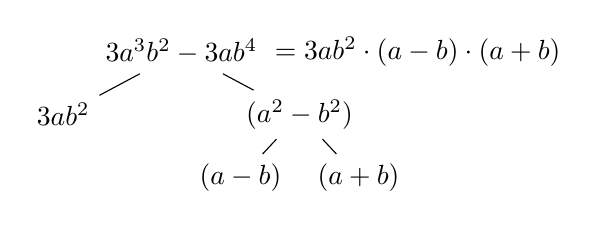
\begin{tikzpicture}[level/.style={sibling distance=30mm/#1, level distance=8mm}]
% \node {$ \qquad \qquad \qquad \qquad \qquad 
%         3a^{3}b^{2}-3ab^{4} = 3ab^2 \cdot (a-b) \cdot (a+b)$}
\node {$3a^{3}b^{2}-3ab^{4}$}
  child {node {$3ab^2$}}
  child {node {$(a^2 -b^2)$}
    child {node {$(a-b)$}}
    child {node {$(a+b)$}}
  };

\draw (3, 0) node {$= 3ab^2 \cdot (a-b) \cdot (a+b)$};
\end{tikzpicture}

\scompfattpol
 \end{center}
\end{inaccessibleblock}
\end{minipage}

Per esempio, scomporre il numero~\(42\) significa scriverlo 
come~\(2\cdot 3 \cdot 7\) dove~\(2\),~\(3\) e~\(7\) sono i suoi fattori primi.
Anche~\(42 = 6 \cdot 7\) è una scomposizione, ma non è in fattori primi. 
Allo stesso modo un polinomio va scomposto in fattori non ulteriormente
scomponibili che si chiamano \emph{irriducibili}. 
%(questa dovrebbe andare a sinistra della tabella)

Si può verificare che \(3ab^{2}(a-b)(a+b)\) è una scomposizione in fattori di
\(3a^{3}b^{2}-3ab^{4}\) eseguendo le moltiplicazioni:
\[3ab^{2}(a-b)(a+b)=3ab^{2}(a^{2}+ab-ba-b^{2})=
  3ab^{2}\tonda{a^{2}-b^{2}}=3a^{3}b^{2}-3ab^{4}\]
  
La scomposizione termina quando non è possibile scomporre ulteriormente i 
fattori individuati.
Come per i numeri, la scomposizione in fattori dei polinomi identifica il 
polinomio in maniera univoca (a meno di multipli).

\begin{definizione}
Un polinomio si dice \emph{riducibile} (scomponibile) se può essere scritto 
come prodotto di due o più polinomi (detti fattori) di grado maggiore di zero.
In caso contrario esso si dirà \emph{irriducibile}.
\end{definizione}

La caratteristica di un polinomio di essere irriducibile dipende dall'insieme 
numerico al quale appartengono i coefficienti del polinomio;
uno stesso polinomio può essere irriducibile nell'insieme dei numeri 
razionali, ma riducibile in quello dei numeri reali o ancora in quello dei 
complessi.
Dalla definizione consegue che un polinomio di primo grado è irriducibile.

\begin{definizione}
La scomposizione in fattori di un polinomio è la sua scrittura come prodotto 
di fattori irriducibili.
\end{definizione}

Di seguito vedremo alcuni metodi per scomporre in fattori i polinomi.

% \ovalbox{\risolvi \ref{ese:15.1}}

\subsection{Raccoglimento fattore comune}
\label{subsec:divpol_fattorecomune}

\subsubsection{Raccoglimento totale}

Questo è il primo metodo che si deve cercare di utilizzare per scomporre un 
polinomio.
Il metodo si basa sulla proprietà distributiva della moltiplicazione rispetto 
all'addizione.
Prendiamo in considerazione il seguente prodotto:~\(a(x+y+z)=ax+ay+az\).

Il nostro obiettivo è ora quello di procedere da destra verso sinistra, 
cioè avendo il polinomio~\(ax+ay+az\) per individuare il 
prodotto che lo ha generato possiamo osservare che i tre monomi contengono 
tutti la lettera~\(a\), che quindi si può mettere in comune,
o come anche si dice ``in evidenza''. Perciò scriviamo 
\[ax+ay+az=a(x+y+z).\]

 \begin{esempio}
Scomporre in fattori~\(6a^{5}b-15a^{2}b^{3}+3a^2b\).
 \begin{enumeratea}
 \item Trovo tutti i fattori comuni con l'esponente 
minore:~\(\mcd=3a^2b\)
 \item divido ciascun termine del polinomio per \(3a^2b\):
\[6a^{5}b : 3a^2b = 2a^{3}; \quad 
  -15a^{2}b^{3} : 3a^2b = -5b^{2}; \quad 
  +3a^2b : 3a^2b = +1\]
% \begin{multicols}{2}
%    \begin{itemize} [nosep]
%    \item \(6a^{5}b : 3a^2b = 2a^{3}\)
%    \item \(-15a^{2}b^{3} : 3a^2b = -5b^{2}\)
%    \item \(+3a^2b : 3a^2b = +1\)
%    \end{itemize}
% \end{multicols}
 \item quindi:\quad 
\(6a^{5}b-15a^{2}b^{3}+3a^2b=3a^{2}b\tonda{2a^{3}-5b^{2}+1}\)
 \end{enumeratea}
 \end{esempio}

\begin{procedura}
Mettere in evidenza il fattore comune:
\begin{enumeratea}
\item trovare il~\(\mcd\) di tutti i termini che formano il polinomio: tutti i 
 fattori in comune con l'esponente minimo con cui compaiono;
\item scrivere il polinomio come prodotto del~\(\mcd\) per il polinomio 
ottenuto 
 dividendo ciascun monomio del polinomio di partenza per il~\(\mcd\)
\item verificare la scomposizione eseguendo la moltiplicazione per vedere se 
 il prodotto dà come risultato il polinomio di partenza.
\end{enumeratea}
\end{procedura}

% \begin{exrig}
 \begin{esempio}
Scomporre in fattori~\(5a^{2}x^2-10ax^{5}\).
  \begin{enumeratea}
  \item tra i coefficienti numerici il fattore comune è~\(5\), 
   tra la parte letterale sono in comune le lettere~\(a\) con esponente \(1\) 
   e~\(x\) con esponente~\(2\), pertanto il~\(\mcd=5ax^2\)
 \item divido ciascun termine del polinomio per~\(5ax^2\):
 \[5a^{2}x^2:5ax^2=a; \quad -10ax^{5}:5ax^2=-2x^3\]
  \item quindi:\quad \(5a^{2}x^2-10ax^{5}=5ax^2(a-2x^3)\).
  \end{enumeratea}
 \end{esempio}

 \begin{esempio}
Scomporre in fattori~\(10x^{5}y^{3}z-15x^3y^{5}z+5x^2y^{3}z\).
 \begin{enumeratea}
 \item Trovo tutti i fattori comuni con l'esponente 
minore:~\(\mcd=5x^2y^{3}z\)
 \item divido ciascun termine del polinomio per~\(5x^2y^{3}z\):
\[10x^{5}y^{3}z:5x^2y^{3}z=2x^3; \quad
-15x^3y^{5}z:5x^2y^{3}z=-3xy^{2}; \quad
+5x^2y^{3}z:5x^2y^{3}z=+1\]
 \item quindi:\quad \(10x^{5}y^{3}z-15x^3y^{5}z+5x^2y^{3}z =
 5x^2y^{3}z \cdot (2x^3-3xy^{2}+1)\)
 \end{enumeratea}
 \end{esempio}

% \osservazione La scomposizione in fattori riguarda la moltiplicazione e la 
%  divisione quindi il terzo termine del polinomio di partenza dà come 
%  risultato~\(1\), non~\(0\).
 
\osservazione Avremmo anche potuto scegliere il fattore da raccogliere 
 con il segno~\((-)\), in questo caso avremmo 
 ottenuto:~\(-5x^2y^{3}z\cdot (-2x^3+3xy^{2}+4z)\).
 
 \begin{esempio}
Scomporre in fattori~\(-8x^2y^{3}+10x^3y^{2}\).
 \begin{enumerate*}
 \item  Se scegliamo come mcd il fattore~\(-2x^2y^{2}\)
  otteniamo~\(-8x^2y^{3}+10x^3y^{2}=-2x^2y^{2}(4y-5x)\)
 \item Se scegliamo come mcd il fattore~\(2x^2y^{2}\)
  otteniamo~\(-8x^2y^{3}+10x^3y^{2}=2x^2y^{2}(-4y+5x)\)
 \end{enumerate*}
 \end{esempio}
% \end{exrig}

Non è detto che il fattore da raccogliere debba essere un numero o una lettera, 
potrebbe essere anche un'espressione comune a più addendi come negli esempi 
seguenti.

% \begin{exrig}

 \begin{esempio}
Scomporre in fattori~\(6a(x-1)+7b(x-1)\).
  \begin{enumeratea}
  \item Il fattore comune è~\((x-1)\); 
  \item dividendo i termini otteniamo:
\[6a(x-1):(x-1)=6a; \quad 7b(x-1):(x-1)=7b\]
  \item quindi: \quad \(6a(x-1)+7b(x-1)=(x-1)(6a+7b)\).
  \end{enumeratea}
 \end{esempio}

 \begin{esempio}
Scomporre in fattori~\(10(x+1)^{2}-5a(x+1)\).
  \begin{enumeratea}
  \item il fattore comune è~\(5(x+1)\);
  \item quindi: \quad 
  \(10(x+1)^{2}-5a(x+1)=5(x+1)\tonda{2(x+1)-a}=5(x+1)\tonda{2x+2-a}\)
  \end{enumeratea}
 \end{esempio}

% \end{exrig}

% \ovalbox{\risolvii \ref{ese:15.2}, \ref{ese:15.3}, \ref{ese:15.4}, 
%  \ref{ese:15.5}, \ref{ese:15.6}, \ref{ese:15.7}, \ref{ese:15.8}, 
%  \ref{ese:15.9}, \ref{ese:15.10},\ref{ese:15.11}, \ref{ese:15.12}, 
%  \ref{ese:15.13}}
% 
% \vspazio\ovalbox{\ref{ese:15.14}}

\subsection{Raccoglimento parziale}
\label{subsec:divpol_raccoglimentoparziale}

Quando un polinomio non ha alcun fattore comune a tutti i suoi termini, 
possiamo provare a mettere in evidenza tra gruppi di monomi
e successivamente individuare il polinomio in comune.

Osserviamo il prodotto~\((a+b)(x+y+z)=ax+ay+az+bx+by+bz\) e
vediamo come è possibile scomporre il polinomio 
\(ax+ay+az+bx+by+bz\).

% \begin{exrig}
 \begin{esempio}
Scomponiamo in fattori~\(ax+ay+az+bx+by+bz\). 

Non c'è nessun fattore comune a tutto il polinomio.

Proviamo a mettere in evidenza per gruppi di termini: tra i primi tre 
raccogliamo \(a\) e tra gli altri tre raccogliamo \(b\) ottenendo:
\(a(x+y+z)+b(x+y+z)\). 

Ora risulta semplice vedere che il trinomio~\((x+y+z)\) è in comune e quindi 
lo possiamo mettere in evidenza. Riassumendo avremo:
\[ax+ay+az+bx+by+bz=a(x+y+z)+b(x+y+z)=(x+y+z)(a+b)\]
 \end{esempio}
% \end{exrig}

\begin{procedura}
Eseguire il raccoglimento parziale.
\begin{enumeratea}
\item Dopo aver verificato che non è possibile effettuare un raccoglimento a 
 fattore comune totale raggruppo i monomi in modo che in ogni gruppo sia 
 possibile mettere in comune qualche fattore;
\item verifico se la nuova scrittura del polinomio ha un polinomio 
 (binomio, trinomio\ldots) comune a tutti i termini;
\item se è presente il fattore comune a tutti i termini lo metto in evidenza;
\item se il fattore comune non è presente la scomposizione è fallita, allora 
 posso provare a raggruppare diversamente i monomi o abbandonare questo metodo.
\end{enumeratea}
\end{procedura}

% \begin{exrig}
 \begin{esempio}
Scomporre in fattori~\(ax+ay+bx+ab\).
  \begin{enumeratea}
  \item Provo a mettere in evidenza la~\(a\) nel primo e secondo termine e 
   la~\(b\) nel terzo e quarto termine:~\(ax+ay+bx+ab=a(x+y)+b(x+a)\)
  \item non c'è nessun fattore comune: il metodo è fallito, il polinomio non 
si può scomporre.
  \end{enumeratea}
 \end{esempio}

% \newpage %-------------------------------------------------

 \begin{esempio}
Scomporre in fattori~\(bx-2ab+2ax-4a^{2}\).
 \begin{enumeratea}
 \item Non vi sono fattori da mettere a fattore comune totale, proviamo con 
  il raccoglimento parziale:~\(b\) nei primi due monomi e~\(2a\) negli altri 
due;
 \item \(\underline{bx} -\underline{2ab}+\underline{\underline{2ax}}-
        \underline{\underline{4a^{2}}}=
        b(\underline{x-2a})+2a(\underline{x-2a})=(x-2a)(b+2a)\).
 \end{enumeratea}
 \end{esempio}

 \begin{esempio}
Scomporre in fattori~\(bx^3+x^2-bx-1+abx+a\).
 \begin{enumeratea}
  \item Raggruppiamo nel seguente 
   modo:~\(\underline{bx^3}+\underline{\underline {x^2}}-\underline{bx}-
          \underline{\underline{1}}+\underline{abx}+\underline{\underline{a}}\) 
   tra quelli con sottolineatura semplice metto a fattore comune~\(bx\), 
   negli altri raccogliamo~\(1\)
  \item
   \(\underline{bx^3}+\underline{\underline {2x^2}}-\underline{bx}-
    \underline{\underline{1}}+\underline{abx}+\underline{\underline{a}}=
    bx\bigl(\underline{x^2-1+a}\bigr)+1\bigl(\underline{x^2-1+a}\bigr)=
    \bigl(x^2+a-1\bigr)\bigl(bx+1\bigr)\).
 \end{enumeratea}
 \end{esempio}

 \begin{esempio}
Scomporre in fattori~\(5ab^{2}-10abc-25abx+50acx\).
 \begin{enumeratea}
  \item Il fattore comune è~\(5a\), quindi:
    \begin{itemize*}
    \item \(5ab^{2}-10abc-25abx+50acx=5a\bigl(b^{2}-2bc-5bx+10cx\bigr)\)
    \end{itemize*}
  \item vediamo se è possibile scomporre il polinomio in parentesi con un 
   raccoglimento parziale~\(5a(\underline{b^{2}}-\underline{2bc}
     -\underline{\underline{5bx}}+\underline{\underline{10cx}})=
     5a\bigl[b(\underline{b-2c})-5x(\underline{b-2c})\bigr]=5a(b-2c)(b-5x)\).
 \end{enumeratea}
 \end{esempio}
% \end{exrig}

% \ovalbox{\risolvii \ref{ese:15.16}, \ref{ese:15.17}, \ref{ese:15.18}, 
% \ref{ese:15.19}, \ref{ese:15.20}, \ref{ese:15.21}, \ref{ese:15.22}, 
% \ref{ese:15.23}, \ref{ese:15.24},\ref{ese:15.25}, \ref{ese:15.26}}
% 
% \ovalbox{\ref{ese:15.27}, \ref{ese:15.28}}

% ----------------- Riconoscimento -------------------------

\subsection{Riconoscimento di prodotti notevoli}
\label{subsec:divpol_prodnot}

Un importante strumento per la scomposizione di polinomi è legato al saper 
riconoscere i prodotti notevoli.
Ogni prodotto notevole mette a disposizione un metodo per scomporre in 
fattori i polinomi.

\subsubsection{Differenza di due quadrati}
\label{subsubsec:divpol_difquad}

Un binomio che sia la differenza dei quadrati di due monomi può essere 
scomposto come prodotto tra la somma dei due monomi (basi dei quadrati) e 
la loro differenza.
\begin{equation*}
(A+B)\cdot (A-B)=
A^{2}-B^{2}\quad \Rightarrow \quad A^{2}-B^{2}=(A+B)\cdot (A-B).
\end{equation*}

% \begin{exrig}
 \begin{esempio}
Scomporre in fattori~\(\dfrac{4}{9}a^{4}-25b^{2}\).
\[\dfrac{4}{9}a^{4}-25b^{2}=
  \tonda{\dfrac{2}{3}a^{2}}^{2}-\tonda{5b}^{2}=
  \tonda{\dfrac{2}{3}a^{2}+5b}\cdot \tonda{\dfrac{2}{3}a^{{2}}-5b}\]
 \end{esempio}

 \begin{esempio}
Scomporre in fattori~\(-x^6+16y^{2}\).
\[-x^6+16y^{2}=-\tonda{x^3}^{2}+\tonda{4y}^{2}=
  \tonda{x^3+4y}\cdot \tonda{-x^3+4y}\]
 \end{esempio}

 \begin{esempio}
Scomporre in fattori~\(a^{2}-\tonda{x+1}^{2}\).
La formula precedente vale anche se~\(A\) e~\(B\) sono polinomi. 
\(a^{2}-\tonda{x+1}^{2}=
 \left[a+(x+1)\right]\cdot \left[a-(x+1)\right]=(a+x+1)(a-x-1)\)
\end{esempio}

 \begin{esempio}
Scomporre in fattori~\(\tonda{2a-b^{2}}^{2}-(4x)^{2}\).
\[\tonda{2a-b^{2}}^{2}-(4x)^{2}=
\tonda{2a-b^{2}+4x}\cdot \tonda{2a-b^{2}-4x}\]
 \end{esempio}

 \begin{esempio}
Scomporre in fattori~\((a+3b)^{2}-(2x-5)^{2}\).
\[(a+3b)^{2}-(2x-5)^{2}=(a+3b+2x-5)\cdot (a+3b-2x+5).\]
 \end{esempio}
% \end{exrig}

Per questo tipo di scomposizioni, la cosa più difficile è riuscire a 
riconoscere un quadrinomio o un polinomio di sei termini come differenza 
di quadrati. Riportiamo i casi principali:
\begin{itemize*}
 \item \((A+B)^{2}-C^{2}=A^{{2}}+2AB+B^{2}-C^{2}\)
 \item \(A^{2}-(B+C)^{2}=A^{2}-B^{2}-2BC-C^{2}\)
 \item \((A+B)^{2}-(C+D)^{2}=A^{2}+2AB+B^{2}-C^{2}-2CD-D^{2}\).
\end{itemize*}

% \begin{exrig}
 \begin{esempio}
Scomporre in fattori~\(4a^{2}-4b^{2}-c^{2}+4bc\).

Gli ultimi tre termini possono essere raggruppati per formare il quadrati di 
un binomio.
 \begin{equation*}
   \begin{split}
     4a^{2}-4b^{2}-c^{2}+4bc &=4a^{2}-\tonda{4b^{2}+c^{2}-4bc} \\
                 &= (2a)^{2}-(2b-c)^{2}=(2a+2b-c)\cdot (2a-2b+c).
   \end{split}
  \end{equation*}
 \end{esempio}

 \begin{esempio}
Scomporre in fattori~\(4x^4-4x^2-y^{2}+1\).
\[4x^4-4x^2-y^{2}+1=\tonda{2x^2-1}^{2}-(y)^{2}=(2x^2-1+y)\cdot 
(2x^2-1-y).\]
 \end{esempio}

 \begin{esempio}
Scomporre in fattori~\(a^{2}+1+2a+6bc-b^{2}-9c^{2}\).
 \begin{equation*}
   \begin{split}
     a^{2}+1+2a+6bc-b^{2}-9c^{2} 
&=\tonda{a^{2}+1+2a}-\tonda{b^{2}+9c^{2}-6{bc}} \\
                 &= (a+1)^{2}-(b-3c)^{2}=(a+1+b-3c)\cdot (a+1-b+3c).
   \end{split}
  \end{equation*}
 \end{esempio}
% \end{exrig}
% \ovalbox{\risolvii \ref{ese:16.29}, \ref{ese:16.30}, \ref{ese:16.31}, 
% \ref{ese:16.32}, \ref{ese:16.33}, \ref{ese:16.34}, \ref{ese:16.35}, 
% \ref{ese:16.36},%
% \ref{ese:16.37}, \ref{ese:16.38}, \ref{ese:16.39}}
% 
% \vspazio\ovalbox{\ref{ese:16.40}, \ref{ese:16.41}}
\subsubsection{Quadrato di un binomio}
\label{subsubsec:divpol_quadbin}

Se abbiamo un trinomio costituito da due termini che sono quadrati di due 
monomi ed il terzo termine è uguale al doppio prodotto
degli stessi due monomi, allora il trinomio può essere scritto sotto forma di 
quadrato di un binomio, secondo il prodotto notevole:
\[(A+B)^{2}=A^{2}+2AB+B^{2}\quad \Rightarrow \quad 
  A^{2}+2AB+B^{2}=(A+B)^{2}\]
\[(A-B)^{2}=A^{2}-2AB+B^{2}\quad \Rightarrow \quad 
  A^{2}-2AB+B^{2}=(A-B)^{2}\]
Poiché il quadrato di un numero è sempre positivo, valgono anche le seguenti 
uguaglianze.
\[(-A-B)^{2}=(A+B)^{2}\quad\Rightarrow\quad 
  A^{2}+2AB+B^{2}=(A+B)^{2}=(-A-B)^{2}\]
\[(-A+B)^{2}=(A-B)^{2}\quad \Rightarrow \quad 
A^{2}-2AB+B^{2}=(A-B)^{2}=(-A+B)^{2}\]

% \begin{exrig}
 \begin{esempio}
Scomporre in fattori~\(4a^{2}+12ab^{2}+9b^{4}\).

Notiamo che il primo ed il terzo termine sono quadrati, rispettivamente 
di~\(2a\) e di~\(3b^{2}\), ed il secondo termine è il doppio prodotto degli 
stessi 
monomi, pertanto possiamo scrivere:
\[4a^{2}+12{ab}^{2}+9b^{4}=(2a)^{2}+2 \cdot (2a) \cdot (3b^{2})+
  \tonda{3b^{2}}^{2}=\tonda{2a+3b^{2}}^{2}=\tonda{-2a-3b^{2}}^{2}\]
 \end{esempio}

 \begin{esempio}
Scomporre in fattori~\(x^2-6x+9\).

Il primo ed il terzo termine sono quadrati, il secondo termine compare con il 
segno ``meno''.
Dunque:~\(x^2-6x+9=x^2-2\cdot 3\cdot x+3^{2}=(x-3)^{2}\), 
ma anche~\(x^2-6x+9=(-x+3)^{2}\).
 \end{esempio}

 \begin{esempio}
Scomporre in fattori~\(x^4+4x^2+4\).

Può accadere che tutti e tre i termini siano tutti quadrati. 
\(x^4+4x^2+4\) è formato da tre quadrati, ma il secondo termine, quello 
di grado intermedio, è anche il doppio prodotto dei due monomi di cui il 
primo ed il terzo termine sono i rispettivi quadrati.
Si ha dunque:
\[x^4+4x^2+4=
  \tonda{x^2}^{2}+2 \cdot (2) \cdot \tonda{x^2}+(2)^{2}=
  \tonda{x^2+2}^{2}=\tonda{-x^2-2}^{2}\]
 \end{esempio}
% \end{exrig}

\begin{procedura}
Individuare il quadrato di un binomio:
\begin{enumeratea}
\item individuare le basi dei due quadrati;
\item verificare se il terzo termine è il doppio prodotto delle due basi;
\item scrivere tra parentesi le basi dei due quadrati e il quadrato fuori 
 dalla parentesi;
\item mettere il segno ``più'' o ``meno'' in accordo al segno del termine che 
 non è un quadrato.
\end{enumeratea}
\end{procedura}

Può capitare che i quadrati compaiano con il coefficiente negativo, ma si può 
rimediare mettendo in evidenza il segno ``meno'' (raccogliendo il fattore 
\(-1\)).

% \begin{exrig}
 \begin{esempio}
Scomporre in fattori~\(-9a^{2}+12{ab}-4b^{2}\).

Mettiamo~\(-1\) a fattore comune
\(-9a^{2}+12ab-4b^{2}=-(9a^{2}-12{ab}+4b^{2})=-(3a-2b)^{2}\).
 \end{esempio}

 \begin{esempio}
Vediamo alcuni esempi svolti operando, dove possibile il raccoglimento a 
fattore comune e poi il riconoscimento del quadrato del binomio.

\begin{enumerate}
\item 
\(-x^4-x^2-\dfrac{1}{4}=-\tonda{x^4+x^2+\dfrac{1}{4}}=
  -\tonda{x^2+\dfrac{1}{2}}^{2}\)
\item 
\(x^2+6xy^{2}-9y^{4}=-\tonda{x^2-6xy^{2}+9y^{4}}=
  -\tonda{x-3y^{2}}^{2}\)
\item 
\(2a^{3}+20a^{2}+50a=2a\tonda{a^{2}+10a+25}=2a\tonda{a+5}^{2}\)
\item 
\(2a^{2}+4a+2=2\tonda{a^{2}+2a+1}=2(a+1)^{2}\)
\item 
\(\dfrac{3}{8}a^{2}+3ab+6b^{2}=
  \dfrac{3}{8}\tonda{a^{2}+8ab+16b^{2} }=
  \dfrac{3}{8}\tonda{a+4b}^{2}\)
\end{enumerate}
\end{esempio}

% \end{exrig}
% \ovalbox{\risolvii \ref{ese:16.1}, \ref{ese:16.2}, \ref{ese:16.3}, 
% \ref{ese:16.4}, \ref{ese:16.5}, \ref{ese:16.6}, \ref{ese:16.7}, 
% \ref{ese:16.8}, \ref{ese:16.9}, \ref{ese:16.10},\ref{ese:16.11}, 
% \ref{ese:16.12}}

\subsubsection{Quadrato di un polinomio}
\label{subsubsec:divpol_quadpol}

Se siamo in presenza di sei termini, tre dei quali sono quadrati, 
verifichiamo se il polinomio è il quadrato di un trinomio secondo le seguenti 
regole.

\begin{equation*}
(A+B+C)^{2}=A^{2}+B^{2}+C^{2}+2AB+2AC+2BC.
\end{equation*}
\begin{equation*}
A^{2}+B^{2}+C^{2}+2AB+2AC+2BC=(A+B+C)^{2}=(-A-B-C)^{2}.
\end{equation*}
Notiamo che i doppi prodotti possono essere tutt'e tre positivi, oppure uno 
positivo e due negativi: indicano se i rispettivi monomi sono concordi o 
discordi.

% \begin{exrig}
 \begin{esempio}
Scomporre in fattori~\(16a^{4}+b^{2}+1+8a^{2}b+8a^{2}+2b\).

I primi tre termini sono quadrati, rispettivamente di~\(4a^{2}\),\(b\) 
e~\(1\), si può verificare poi che gli altri tre termini sono i doppi 
prodotti:~\(16a^{4}+b^{2}+1+8a^{2}b+8a^{2}+2b=\tonda{4a^{2}+b+1}^{2}\).
 \end{esempio}

 \begin{esempio}
Scomporre in fattori~\(x^4+y^{2}+z^{2}-2x^2y-2x^2z+2yz\).
\[x^4+y^{2}+z^{2}-2x^2y-2x^2z+2yz=
  \tonda{x^2-y-z}^{2}=\tonda{-x^2+y+z}^{2}\]
 \end{esempio}

 \begin{esempio}
Scomporre in fattori~\(x^4-2x^3+3x^2-2x+1\).

In alcuni casi anche un polinomio di cinque termini può essere il quadrato di 
un trinomio.
Per far venire fuori il quadrato del trinomio si può scindere il 
termine~\(3x^2\) come somma:
\[3x^2=x^2+2x^2.\]
In questo modo si ha:
\[x^4-2x^3+3x^2-2x+1=x^4-2x^3+x^2+2x^2-2x+1=(x^2-x+1)^{2}\]
 \end{esempio}
% \end{exrig}

Nel caso di un quadrato di un polinomio la regola è sostanzialmente la stessa:
\begin{equation*}
(A+B+C+D)^{2}=A^{2}+B^{2}+C^{2}+D^{2}+2AB+2AC+2AD+2BC+2BD+2CD.
\end{equation*}
% \ovalbox{\risolvii \ref{ese:16.13}, \ref{ese:16.14}, \ref{ese:16.15}, 
% \ref{ese:16.16}, \ref{ese:16.17}, \ref{ese:16.18}, \ref{ese:16.19}}

\subsubsection{Cubo di un binomio}
\label{subsubsec:divpol_cubobin}

I cubi di binomi sono di solito facilmente riconoscibili. Un quadrinomio è lo 
sviluppo del cubo di un binomio se due suoi termini sono i cubi di due monomi 
e gli altri due termini sono i tripli prodotti tra uno dei due monomi ed il 
quadrato dell'altro, secondo le seguenti formule.
\[(A+B)^{3}=A^{3}+3A^{2}B+3AB^{2}+B^{3}\quad \Rightarrow \quad 
A^{3}+3A^{2}B+3AB^{2}+B^{3}=(A+B)^{3}\]
\[(A-B)^{3}=A^{3}-3A^{2}B+3AB^{2}-B^{3}\quad \Rightarrow \quad 
A^{3}-3A^{2}B+3AB^{2}-B^{3}=(A-B)^{3}\]
\[(-A+B)^{3}=-A^{3}+3A^{2}B-3AB^{2}+B^{3}\quad \Rightarrow \quad 
-A^{3}+3A^{2}B-3AB^{2}+B^{3}=(-A+B)^{3}\]
\[(-A-B)^{3}=-A^{3}-3A^{2}B-3AB^{2}-B^{3}\quad \Rightarrow \quad 
-A^{3}-3A^{2}B-3AB^{2}-B^{3}=(-A-B)^{3}\]
Per il cubo non si pone il problema, come per il quadrato, del segno della 
base, perché un numero, elevato ad esponente dispari, se è positivo rimane 
positivo, se è negativo rimane negativo.

% \begin{exrig}
 \begin{esempio}
Scomporre in fattori~\(8a^{3}+12a^{2}b+6{ab}^{2}+b^{3}\).

Notiamo che il primo ed il quarto termine sono cubi, rispettivamente 
di~\(2a\) e di~\(b\), 
il secondo termine è il triplo prodotto tra il quadrato di~\(2a\) e~\(b\), 
il terzo è il triplo prodotto tra~\(2a\) e il quadrato di~\(b\).
Abbiamo dunque:
\[8a^{3}+12a^{2}b+6ab^{2}+b^{3}=
  (2a)^{3}+3\cdot (2a)^{2}\cdot (b)+3\cdot (2a)\cdot (b)^{2}=(2a+b)^{3}\]
 \end{esempio}

 \begin{esempio}
Scomporre in fattori~\(-27x^3+27x^2-9x+1\).

Le basi del cubo sono il primo e il quarto termine, rispettivamente cubi 
di~\(-3x\) e di~\(1\).
Dunque:
\[-27x^3+27x^2-9x+1=
  (-3x)^{3}+3\cdot (-3x)^{2}\cdot 1+3\cdot (-3x)\cdot 1^{2}+1=(-3x+1)^{3}\]
 \end{esempio}

 \begin{esempio}
Scomporre in fattori~\(x^6-x^4+\dfrac{1}{3}x^2-\dfrac{1}{27}\).

Le basi del cubo sono~\(x^2\) e~\(-\dfrac{1}{3}\) i termini centrali sono i 
tripli prodotti, quindi~\(\tonda{x^2-\dfrac{1}{3}}^{3}\).
\end{esempio}
% \end{exrig}
% \ovalbox{\risolvii \ref{ese:16.20}, \ref{ese:16.21}, \ref{ese:16.22}, 
% \ref{ese:16.23}, \ref{ese:16.24},\ref{ese:16.25}, \ref{ese:16.26}, 
% \ref{ese:16.27}, \ref{ese:16.28}}



% ----------------- Altre tecniche -------------------------


% \chapter{}
\subsection{Altre tecniche di scomposizione}
\label{subsec:divpol_altretecniche}

\subsubsection{Trinomi particolari}
\label{subsubsec:trinpart}

Consideriamo il seguente prodotto:
\[(x+3)(x+2)=x^2+2x+3x+3 \cdot 2=x^2+(2+3)x+6=x^2+5x+6.\]
Poniamoci ora l'obiettivo opposto: se abbiamo il
polinomio~\(x^2+5x+6\) come facciamo a trovare ritrovare il prodotto
che lo ha originato? Possiamo notare che il~5 deriva dalla somma tra
il~3 e il~2, mentre il~6 deriva dal prodotto tra~3 e~2. Generalizzando:
\[\tonda{x+A}\cdot \tonda{x+B}=
  x^{{2}}+Ax+Bx+AB=x^2+\tonda{A+B}x+A\cdot B\]
Leggendo la formula precedente da destra verso sinistra:
\[x^{{2}}+\overset{S}{\tonda{A+B}}x+\overset{P}{A \cdot B}
=\tonda{x+A}\cdot\tonda{x+B}\]
Possiamo allora concludere che se abbiamo un trinomio di secondo grado
in una sola lettera, a coefficienti interi, avente il termine di
secondo grado con coefficiente~\(1\), se riusciamo a trovare due numeri~\(A\) 
e~\(B\) tali che la loro somma (\(S\)) sia uguale al
coefficiente del termine di primo grado ed il loro prodotto (\(P\)) sia 
uguale al termine noto, allora il polinomio è scomponibile nel 
prodotto~\((x+A)(x+B)\).

Osserva che il termine noto, poiché è dato dal prodotto dei numeri
che cerchiamo, ci dice se i due numeri sono concordi o discordi.
Inoltre, se il numero non è particolarmente grande è sempre
possibile scrivere facilmente tutte le coppie di numeri che danno come
prodotto il numero cercato, tra tutte queste coppie dobbiamo poi
individuare quella che ha per somma il coefficiente del termine di
primo grado.

% \begin{exrig}
 \begin{esempio}
 \(x^2+\overset{S}{7}x+\overset{P}{12}\)

I coefficienti sono positivi e quindi i due numeri da trovare sono
entrambi positivi.
Il termine noto~\(12\) può essere scritto sotto forma di prodotto di due
numeri naturali solo come:
\[12\cdot 1;\quad~6\cdot 2;\quad~3\cdot 4\]
Le loro somme sono rispettivamente~\(13\), \(8\), \(7\). 
La coppia di numeri che dà per somma \(S=+7\) e prodotto \(P=+12\) è 
pertanto~\(+3\) e~\(+4\). 
Dunque il trinomio si scompone come:

\[x^2+7x+12=\tonda{x+4} \cdot \tonda{x+3}\]
 \end{esempio}

 \begin{esempio}
 \(x^2-\overset{S}{8}x+\overset{P}{15}\)

vediamo che i due numeri cercati dovranno avere 
prodotto positivo e somma negativa, quindi saranno entrambi negativi. 
% Dobbiamo cercare due numeri negativi la cui somma sia~\(-8\) e il cui 
% prodotto sia~\(+15\). 
Le coppie di numeri negativi che danno~\(+15\) come prodotto sono \(-15\) 
\(-1\) e~\(-5\) \(-3\).
I due numeri cercati sono~\(-5\) e~\(-3\) e il trinomio si scompone come:
\[x^2-8x+15=\tonda{x-5}\cdot \tonda{x-3}.\]
 \end{esempio}

% \newpage %----------------------------------------

\begin{esempio}
 \(x^2+\overset{S}{4}x-\overset{P}{5}\)

Abbiamo che \(P = -5 = A \cdot B = (-5) \cdot (+1) = (+5) \cdot (-1)\).

Dato che \(S = +4\) il polinomio si scompone:
\[x^2+4x-5=\tonda{x+5}\cdot \tonda{x-1}\]
\end{esempio}

\begin{esempio}
 \(x^2-\overset{S}{3}x-\overset{P}{10}\)

Le coppie di numeri il cui prodotto è~\(P=-10\) sono:
\(\{\punto{+5}{-2};~\punto{-5}{+2}\}\).

Dato che~\(S=-3\), la scomposizione sarà:
\[x^2-3x-10=\tonda{x-5}\cdot \tonda{x+2}\]
\end{esempio}

\begin{esempio}
 In alcuni casi si può applicare questa regola anche quando il trinomio
non è di secondo grado, è necessario però che il termine di grado
intermedio sia esattamente di grado pari alla metà di quello di grado
maggiore.

\begin{itemize*}
\item \(x^4+5x^2+6=\tonda{x^2+3}\cdot \tonda{x^2+2}\)
\item \(x^6+x^3-12=\tonda{x^3+4}\cdot \tonda{x^3-3}\)
\item \(a^{4}-10a^{2}+9=\tonda{a^{2}-9}\cdot\tonda{a^{2}-1}=
       \tonda{a+3}\cdot \tonda{a-3}\cdot 
       \tonda{a+1}\cdot\tonda{a-1}\)
\item \(-x^4-x^2+20=-\tonda{x^4+x^2-20}=
       -\tonda{x^2+5}\cdot\tonda{x^2-4}=
       -\tonda{x^2+5}\cdot\tonda{x+2}\cdot \tonda{x-2}\)
\item \(2x^{5}-12x^3-14x=2x\cdot \tonda{x^4-6x^2-7}=2x\cdot%
\tonda{x^2-7}\cdot \tonda{x^2+1}\)
\item \(-2a^{7}+34a^{5}-32a^{3}=-2a^{3}\tonda{a^{4}-17a^{2}+16}
    =-2a^{3}\tonda{a^{2}-1}\tonda{a^{2}-16}\\
=-2a^{3}\tonda{a-1}\tonda{a+1}\tonda{a-4}\tonda{a+4}\)
\end{itemize*}
\end{esempio}

% \end{exrig}

È possibile applicare questo metodo anche quando il
polinomio è in due variabili.

% \begin{exrig}
 \begin{esempio}
 \(x^2+5xy+6y^{2}\).

 Per capire come applicare la regola precedente, possiamo scrivere il
trinomio in questo modo:~\(x^2+\overset{S}{5}xy+\overset{P}{6}y{^{2}}\).

Bisogna cercare due monomi~\(A\) e~\(B\) tali che~\(A+B=5y\)
e~\(A\cdot B=6y^{2}\). Partendo dal fatto che i due numeri che danno~5
come somma e~6 come prodotto sono~\(+3\) e~\(+2\), i monomi cercati 
sono~\(+3y\) e~\(+2y\), infatti~\(+3y+3y=+5y\) e~\(+3y\cdot (+2y)=+6y^{2}\). 
Pertanto si può scomporre come segue:~\(x^2+5xy+6y^{2}=(x+3y)(x+2y)\).
 \end{esempio}
% \end{exrig}

La regola, opportunamente modificata, vale anche se il primo
coefficiente non è~1. Vediamo un esempio.

% \begin{exrig}
 \begin{esempio}
 \(ax^2+bx+c=2x^2-3x+1\).

Non possiamo applicare la regola del trinomio caratteristico dato che 
\(a=2\).
% Con un accorgimento, possiamo riscrivere il polinomio in un altro modo. 
Dobbiamo trovare due numeri \(m\) e \(n\) il cui prodotto sia uguale al 
prodotto sia: \(P = a \cdot c = 2 \cdot 1 = 2\)
e la somma sia: \(S = b = -3\).
In questo esempio: \(m = -2\) e \(n = -1\).
A questo punto spezziamo il monomio centrale nella somma di due monomi in 
questo modo
\[2x^2-3x+1=2x^2\underbrace{-2x-x}_{-3x}+1.\]

Ora possiamo applicare il raccoglimento a fattore comune parziale
\[2x^2-x-1=
% \underbrace{2x^2-2x}_{2x}~\underbrace{-x+1}_{-1}=
\underline{2x^2-2x}~\underline{-x+1}=
2x \cdot \underline{\tonda{x-1}}-1 \cdot \underline{\tonda{x-1}}=
\tonda{x-1}\cdot \tonda{2x-1}.\]
 \end{esempio}
% \end{exrig}

\begin{procedura}
Sia da scomporre un trinomio di secondo grado a coefficienti 
interi~\(ax^2+bx+c\)
% con~\(a\neq~1\)
, cerchiamo due numeri~\(m\) ed~\(n\) tali che: \quad 
\(m \cdot n = a \cdot c\) \quad 
e \quad 
\(m+n=b\)  \quad
se riusciamo a trovarli, li useremo per dissociare
il coefficiente~\(b\) e riscrivere il polinomio nella 
forma~\(p=ax^2+\tonda{m+n}\cdot x+c\)
su cui poi eseguire un raccoglimento parziale.
\end{procedura}

% \ovalbox{\risolvii \ref{ese:17.1}, \ref{ese:17.2}, \ref{ese:17.3}, 
% \ref{ese:17.4}, \ref{ese:17.5}, \ref{ese:17.6}, \ref{ese:17.7}, 
% \ref{ese:17.8}, \ref{ese:17.9}, \ref{ese:17.10}}

\subsubsection{Scomposizione con la regola Ruffini}
\label{subsubsec:divpol_scompruff}

Anche il teorema e la regola di Ruffini aiutano a scomporre in fattori i 
polinomi.

Chiamiamo \emph{zeri} di un polinomio o \emph{zeri} di una funzione in 
una variabile, i valori \(k\) che, se sostituiti alla variabile annullano il 
valore del polinomio o della funzione. 

Il teorema di Ruffini dice che:

\begin{center}
\emph{Se \(k\) è uno zero del polinomio \(P(x)\), allora  
\(P(x)\) è divisibile per \(\tonda{x-k}\).}
\end{center}

Quindi se conosciamo uno zero del polinomio, allora lo possiamo 
scomporre nel prodotto: \(P(x) = \tonda{x-k} \cdot Q(x)\), 
dove~\(Q(x)\) è il quoziente della divisione tra~\(P(x)\) e~\((x-k)\).

\begin{procedura}
Per scomporre un polinomio \(P(x)\), possiamo:
\begin{enumeratea}
\item trovare uno zero: \(k\);
\item calcolare il quoziente \(Q(x)\) della divisione per \(x-k\);
\item scomporre nel prodotto: \(P(x) = \tonda{x-k} \cdot Q(x)\).
\end{enumeratea}
\end{procedura}

Gli \emph{zeri} di un polinomio vengono anche detti \emph{radici del polinomio}.

Gli zeri (o radici) di un polinomio a coefficienti interi, non vanno cercati 
andando a casaccio, ma abbiamo degli elementi per restringere il campo di 
ricerca: 
\emph{le radici intere del polinomio vanno cercate tra i divisori del 
termine noto}.

% \begin{exrig}
 \begin{esempio}
 \(p(x)=x^3+x^2-10x+8\).
 \end{esempio}
Le radici intere del polinomio sono da ricercare nell'insieme dei divisori di 
\(8\), precisamente in~\(\{\pm~1;\pm~2;\pm~4;\pm~8\}\).
Sostituiamo uno alla volta questi numeri nel polinomio, finché non troviamo 
quello che lo annulla.\\
Per~\(x=-1\) si ha~\(P(-1)=(-1)^{3}+(-1)^{2}-10\cdot (-1)+8=-1+1+10+8=18\),\\
Per~\(x=+1\) si ha~\(P(+1)=(+1)^{3}+(+1)^{2}-10\cdot (+1)+8=1+1-10+8=0\),\\
Dato che \(+1\) è uno zero del polinomio, il polinomio è divisibile 
per~\(x-1\).

Usiamo la regola di Ruffini per eseguire la divisione:
\(\tonda{x^3+x^2-10x+8} : \tonda{x-1}\).

\begin{wrapfloat}{figure}{l}{0pt}
% \input{\folder lbr/fig031_rufi.pgf}
\scompruffiniaa
\end{wrapfloat}

% Predisponiamo una griglia come quella a fianco, al primo rigo mettiamo i
% coefficienti di~\(P(x)\), al secondo rigo mettiamo come primo numero la
% radice che abbiamo trovato, cioè~1. Poi procediamo come abbiamo già
% indicato per la regola di Ruffini.
% I numeri che abbiamo ottenuto nell'ultimo rigo sono i
% coefficienti del quoziente: \(q(x)=x^2+2x-8\).

Il quoziente è: \(Q(x)=x^2+2x-8\) e il resto, ovviamente, \(R=0\).\\
Possiamo allora scrivere:
\[x^3+x^2-10x+8=\tonda{x-1}\cdot \tonda{x^2+2x-8}\]

\begin{wrapfloat}{figure}{r}{0pt}
% \input{\folder lbr/fig031_rufi.pgf}
\scompruffiniac
\end{wrapfloat}

Possiamo usare lo stesso metodo per fattorizzare il quoziente: 
\(P_1(x)=x^2+2x-8\). 
Uno zero di questo polinomio è: \(+2\). 
Usiamo ancora il metodo di Ruffini per dividere: 
\(\tonda{x^2+2x-8} : \tonda{x-2}\).
Possiamo farlo prolungando lo schema di Ruffini, come mostrato qui a fianco.

Il nuovo quoziente è: \(x+4\), quindi la scomposizione del polinomio di 
partenza sarà:
\[p(x)=x^3+x^2-10x+8 = \tonda{x-1} \tonda{x-2} \tonda{x+4}\]

% \newpage %------------------------------------------------------

\begin{esempio}
\(x^4-5x^3-7x^2+29x+30\)

Le radici intere vanno cercate tra i divisori di~30, precisamente 
in:
\begin{center}
\(\{\pm~1\) \(\pm~2\) \(\pm~3\) \(\pm~5\) \(\pm~6\) \(\pm~10\)
\(\pm~15\) \(\pm~30\}\)
\end{center}
Sostituiamo questi numeri al posto della~\(x\), finché non troviamo la 
radice\dots\\
per~\(x=1\) si ha: \quad \(P(1)=1-5-7+29+30\), \\
senza effettuare il calcolo si nota 
che i numeri positivi superano quelli negativi, quindi~1 non è una radice,
invece:

\affiancati{.48}{.48}
{
\scompruffiniad
}
{
per~\(x=-1\) si ha:\\
\(P(-1)=+1+5-7-29+30=0\)

Eseguendo la divisione per \(x+1\), otteniamo come primo quoziente: \\
\(P_1=x^3-6x^2-x+30\).

Uno zero di questo nuovo polinomio è: \(x-2\).\\
Eseguiamo una nuova divisione, questa volta per: \(x+2\),
ottenendo come nuovo quoziente:\\
\(P_2=x^2-8x+15\). 

Un suo zero è: \(x=+3\).\\
Eseguiamo una nuova divisione, questa volta per: \(x-3\).
}
\end{esempio}

Non sempre è possibile scomporre un polinomio utilizzando solo numeri
interi. In alcuni casi possiamo provare con le frazioni, in particolare
quando il coefficiente del termine di grado maggiore non è~1. In
questi casi possiamo cercare la radice del polinomio tra le frazioni
del tipo~\(\dfrac{p}{q}\), dove~\(p\) è un divisore del termine noto e~\(q\) 
è un divisore del coefficiente del termine di grado maggiore.

\begin{esempio}
\(6x^2-x-2\)

Determiniamo prima di tutto l'insieme nel quale
possiamo cercare le radici del polinomio. Costruiamo tutte le frazioni
del tipo~\(\dfrac{p}{q}\), con~\(p\) divisore di~\(-2\) e~\(q\) divisore 
di~\(6\). I
divisori di~2 sono~\(\{\pm~1;\pm~2\}\) 
mentre i divisori di~6 sono~\(\{\pm~1;\pm~2;\pm~3;\pm~6\}\).
Le frazioni tra cui cercare sono:
\[\left\{
\pm \dfrac{1}{1};~\pm \dfrac{1}{2};~\pm \dfrac{1}{3};~\pm \dfrac{1}{6};~
\pm \dfrac{2}{1};~\pm \dfrac{2}{2};~\pm \dfrac{2}{3};~\pm \dfrac{2}{6}\right\}\]
cioè i numeri razionali: \quad
\(\left\{
\pm \dfrac{1}{6};~\pm \dfrac{1}{3};~\pm \dfrac{1}{2};~\pm \dfrac{2}{3};~
\pm 1;~\pm 2 \right\}\)

Si ha: \quad \(A(1)=-3; \quad A(-1)=5; \quad A\tonda{\dfrac{1}{2}}=-1; 
       \quad A\tonda{-\dfrac{1}{2}}=0\).
       
Applichiamo la regola di Ruffini per trovare il quoziente.

% \begin{wrapfloat}{figure}{l}{0pt}
% % \input{\folder lbr/fig034_rufi.pgf}
% \end{wrapfloat}

\affiancati{.58}{.38}
{
Dividiamo il polinomio per~\(\tonda{x+\dfrac{1}{2}}\) e otteniamo che:
\vspace{-2mm}
\[6x^2-x-2 = \tonda{6x-4} \cdot \tonda{x+\dfrac{1}{2}}\]
}
{
% \begin{center} 
\hspace{5mm} \scompruffinid 
% \end{center}
}
Mettendo a fattore comune~2 nel primo binomio si ha:
\[6x^2-x-2\ =
\ (6x-4)\cdot \tonda{x+\dfrac{1}{2}}\ =
\ 2(3x-2)\tonda{x+\dfrac{1}{2}}\ =(3x-2)(2x+1)\]
\end{esempio}

% \end{exrig}

% \ovalbox{\risolvii \ref{ese:17.11}, \ref{ese:17.12}, \ref{ese:17.13}, 
% \ref{ese:17.14}, \ref{ese:17.15}}

%%%%%%%%%%%%%%%%%%%%%%%%%%%%%%%%%%%% binomio omogeneo

\subsubsection{Binomi omogenei}
\label{subsubsec:divpol_binomo}

Un binomio omogeneo è un binomio del tipo~\(x^{n} \mp a^{n}\).
Vediamo come scomporlo a seconda del valore di \(n\).

\begin{itemize*}
\item \(n=1\)
 \begin{itemize*}
  \item \(x+a\) è irriducibile perché di primo grado.
  \item \(x-a\) è irriducibile perché di primo grado.
 \end{itemize*}

 \item \(n=2\)
 \begin{itemize*}
  \item \(x^2+a^2\) è irriducibile.
  \item \(x^2-a^2=(x-a)(x+a)\) .
 \end{itemize*}

 \item \(n=3\)
 \begin{itemize*}
  \item 
\affiancati{.59}{.39}{
\(x^3+a^3\) è divisibile per \((x+a)\),\\ 
usando la regola di Ruffini otteniamo:\\[1em]
\(x^3+a^3=(x+a)(x^2-ax+a^2)\)
}{
   \begin{inaccessibleblock}
    [Divisione \((x^3+a^3):(x+a)\) con la regola di Ruffini]
    \begin{center} \binomogeneiruffinia \end{center}
    \end{inaccessibleblock}
}
  \item 
\affiancati{.59}{.39}{
\(x^3-a^3\) è divisibile per \((x-a)\),\\ 
usando la regola di Ruffini otteniamo:\\[1em]
\(x^3-a^3=(x-a)(x^2+ax+a^2)\)
}{
   \begin{inaccessibleblock}
    [Divisione \((x^3-a^3):(x-a)\) con la regola di Ruffini]
    \begin{center} \binomogeneiruffinib \end{center}
    \end{inaccessibleblock}
}
 \end{itemize*}

 \item \(n=4\)
 \begin{itemize*}
  \item \(x^4+a^4\) lo si può scomporre usando un trucco: 
   aggiungere e togliere:~\(-2x^2a^2\).
   
   \(x^4+a^4 = x^4+2x^2b^2+a^4-2x^2a^2 = (x^2+a^2)^2-2x^2a^2=\)
   
   \(\tonda{x^2+a^2-\sqrt{2}xa}\tonda{x^2+a^2+\sqrt{2}xa}\)
   
  \item \(x^4-a^4\) si può scomporre trattandolo come la differenza di due 
   quadrati:
   
   \(x^4-a^4 = (x^2-a^2)(x^2+a^2) = (x-a)(x+a)(x^2+a^2) \)
 \end{itemize*}

 \item \(n=5\)
 \begin{itemize*}
  \item \(x^5+a^5\) è divisibile per \((x+a)\) usando la regola di Ruffini
   ottenendo: 
   
   \(x^5+a^5=(x+a)(x^4-ax^3+x^2a^2-xa^3+a^4)\)
   
  \item \(x^5-a^5\) è divisibile per \((x-a)\) usando la regola di Ruffini
   ottenendo: 
   
   \(x^5-a^5=(x-a)(x^4+ax^3+x^2a^2+xa^3+a^4)\)
   
 \end{itemize*}

 \item \(n=6\) ...
 
\end{itemize*}

% % \begin{exrig}
%  \begin{esempio}
%  \(x^3-8\).
% \end{esempio}
% Il polinomio si annulla per~\(x=2\), che è la radice cubica di~8.
% Calcoliamo il quoziente.
% \begin{wrapfloat}{figure}{l}{0pt}
%  \input{\folder lbr/fig035_rufi.pgf}
% \diffcubia
% \end{wrapfloat}
% Il polinomio quoziente è~\(Q(x)=x^2+2x+4\) e la scomposizione risulta
% \[x^3-8\ =\ (x-2)(x^2+2x+4).\]
% 
% Notiamo che il quoziente assomiglia al quadrato di un binomio, ma non lo
% è in quanto il termine intermedio è il prodotto e non il doppio
% prodotto dei due termini, si usa anche dire che è un ``falso quadrato''.
% Un trinomio di questo tipo non è ulteriormente scomponibile.
% 
% 
%  \begin{esempio}
%  \(x^3+27\).
%  \end{esempio}
%  \begin{wrapfloat}{figure}{l}{0pt}
%  \input{\folder lbr/fig036_rufi.pgf}
% \diffcubib
% \end{wrapfloat}
% Il polinomio si annulla per~\(x=-3\), cioè~\(P(-3)=(-3)^{3}+27=-27+27=0\).
% Il polinomio quindi è divisibile per~\(x+3\). Calcoliamo il quoziente
% attraverso la regola di Ruffini.
% 
% Il polinomio quoziente è~\(Q(x)=x^2-3x+9\) e la scomposizione risulta
% \[x^3+27=(x+3)(x^2-3x+9).\]
% 
% % \end{exrig}
% 
% In generale possiamo applicare le seguenti regole per la scomposizione
% di somma e differenza di due cubi:
% 
% \[A^{3}+B^{3}=(A+B)(A^{2}-AB+B^{2}),\]
% \[A^{3}-B^{3}=(A-B)(A^{2}+AB+B^{2}).\]
% 
% \ovalbox{\risolvii \ref{ese:17.16}, \ref{ese:17.17}, \ref{ese:17.18}}

\subsection{Scomposizione mediante metodi combinati}
\label{subsec:divpol_metodicombinati}

Nei paragrafi precedenti abbiamo analizzato alcuni metodi per ottenere
la scomposizione in fattori di un polinomio e talvolta abbiamo mostrato
che la scomposizione si ottiene combinando metodi diversi.
Sostanzialmente non esiste una regola generale per la scomposizione di
polinomi, cioè non esistono criteri di divisibilità semplici come
quelli per scomporre un numero nei suoi fattori primi. In questo
paragrafo vediamo alcuni casi in cui si applicano vari metodi combinati
tra di loro.

Un buon metodo per ottenere la scomposizione è procedere tenendo conto
di questi suggerimenti:


\begin{enumerate}
\item analizzare se si può effettuare \emph{un raccoglimento totale};
\item \emph{contare il numero di termini} di cui si compone il polinomio:
 \begin{enumerate}
  \item con \emph{due} termini analizzare se il binomio è
   \begin{enumerate}
	\item una \emph{differenza di quadrati} 
	 \(A^{2}-B^{2}=(A-B)(A+B)\)
	\item una \emph{differenza di cubi}
	 \(A^{3}-B^{3}=(A-B)\tonda{A^{2}+AB+B^{2}}\)
	\item una \emph{somma di cubi} 
	 \(A^{3}+B^{3}=(A+B)\tonda{A^{2}-AB+B^{2}}\)
	\item una \emph{somma di quadrati} nel qual caso è \emph{irriducibile} 
	 \(A^{2}+B^{2}\).
   \end{enumerate}
  \item con \emph{tre} termini analizzare se è
   \begin{enumerate}
	\item un \emph{quadrato di binomio} 
	 \(A^{2}\pm~2AB+B^{2}=\tonda{A\pm B}^{2}\)
	\item un \emph{trinomio particolare} del tipo~\(x^2+Sx+P=(x+a)(x+b)\) 
	 con~\(a+b=S\) e~\(a\cdot b=P\)
	\item un \emph{falso quadrato}, che è irriducibile~\(A^{2}\pm AB+B^{2}\).
   \end{enumerate}
  \item con \emph{quattro} termini analizzare se è
   \begin{enumerate}
	\item un \emph{cubo di binomio} 
	 \(A^{3}\pm~3A^{2}B+3AB^{2}\pm B^{3}=\tonda{A\pm B}^{3}\)
	\item una \emph{particolare differenza di quadrati}
	 \subitem \(A^{2}\pm~2AB+B^{2}-C^{2}=(A\pm B+C)(A\pm B-C)\)
	\item un \emph{raccoglimento parziale} \(ax+bx+ay+by=(a+b)(x+y)\).
   \end{enumerate}
  \item con \emph{sei} termini analizzare se è
   \begin{enumerate}
	\item un \emph{quadrato di trinomio} 
	 \(A^{2}+B^{2}+C^{2}+2AB+2{AC}+2{BC}=\tonda{A+B+C}^{2}\)
	\item un \emph{raccoglimento parziale}
	 \subitem \(ax+{bx}+{cx}+{ay}+{by}+{cy}=(a+b+c)(x+y)\).
   \end{enumerate}
  \end{enumerate}
 \item se non riuscite ad individuare nessuno dei casi precedenti, provate ad 
  applicare la \emph{regola di Ruffini}.
\end{enumerate}


% Ricordiamo infine alcune formule per somma e differenza di potenze
% dispari.
% 
% \[A^5+B^5=(A+B)\tonda{A^4-A^3B+A^2B^2-AB^3+B^4},\]
% \[A^5-B^5=(A-B)\tonda{A^4+A^3B+A^2B^2+AB^3+B^4},\]
% \[A^{7}\pm B^{7}=
% (A\pm B)\tonda{A^{6}\mp A^{5}B+A^{4}B^{2}\mp 
% A^{3}B^{3}+A^{2}B^{4}\mp AB^{5}+B^{6}},\]
% \begin{equation*}
% \begin{split}
%  (A^{11}-B^{11})=(A-B)(A^{10}+A^{9}B+A^{8}B^{2}&+A^{7}B^{3}+A^{6}B^{4}\\
%  &+A^{5}B^{5}+A^{4}B^{6}+A^{3}B^{7}+A^{2}B^{8}+AB^{9}+B^{10}).\\
% \end{split}
% \end{equation*}
% 
% La differenza di due potenze ad esponente pari (uguale o diverso)
% rientra nel caso della differenza di quadrati:
% 
% \[A^{8}-B^{10}=\tonda{A^{4}-B^{5}}\tonda{A^{4}+B^{5}}.\]
% 
% In alcuni casi si può scomporre anche la somma di potenze pari:
% 
% \[A^{6}+B^{6}=\tonda{A^{2}}^{3}+\tonda{B^{2}}^{3}=
%   \tonda{A^{2}+B^{2}}\tonda{A^{4}-A^{2}B^{2}+B^{4}},\]
% \[A^{10}+B^{10}=\tonda{A^{2}}^{5}+\tonda{B^{2}}^{5}=
%   \tonda{A^{2}+B^{2}}\tonda{A^{8}-A^{6}B^{2}+A^{4}B^{4}-
%   A^2B^6+B^8}\]
% 
% Proponiamo di seguito alcuni esercizi svolti o da completare in modo che
% possiate acquisire una certa abilità nella scomposizione di polinomi.

% \begin{exrig}

\newpage %--------------------------------------------------

 \begin{esempio}
 \(a^{2}x+5abx-36b^{2}x\).

Il polinomio ha~3 termini, è di terzo grado in~2 variabili, è omogeneo;
tra i suoi monomi si ha~\(\mcd= x\) effettuiamo il raccoglimento
totale:~\(x\cdot\tonda{a^{2}+5ab-36b^{2}}\).
Il trinomio ottenuto come secondo fattore è di grado~2 in~2 variabili,
omogeneo e può essere riscritto
\[a^{2}+\tonda{5b}\cdot a-36b^{2}.\]
Proviamo a scomporlo come trinomio particolare:
cerchiamo due monomi~\(m\) ed~\(n\) tali che~\(m+n=5b\)
e~\(m\cdot n=-36b^{2}\) i due monomi sono~\(m=9b\)
ed~\(n=-4b\)

\[a^{2}x+5abx-36b^{2}x=x\cdot\tonda{a+9b}\cdot \tonda{a-4b}.\]
 \end{esempio}

 \begin{esempio}
 \(x^2+y^{2}+2xy-2x-2y\).

Facendo un raccoglimento parziale del coefficiente~2 tra gli ultimi tre monomi 
perché otterremmo~\(x^2+y^{2}+2\cdot\tonda{xy-x-y}\) su cui non possiamo
fare alcun ulteriore raccoglimento.

I primi tre termini formano però il quadrato di un binomio e tra gli
altri due possiamo raccogliere~\(-2\), quindi
\(\tonda{\underline{{x+y}}}^{2}-2\cdot\tonda{\underline{{x+y}}}\),
raccogliendo~\((x + y)\) tra i due termini si ottiene

\begin{equation*}
x^2+y^{2}+2xy-2x-2y=\tonda{x+y}\cdot \tonda{x+y-2}.
\end{equation*}
 \end{esempio}

 \begin{esempio}
 \(8a+10b+\tonda{1-4a-5b}^{2}-2\).

Tra i monomi sparsi possiamo raccogliere~2 a fattore comune
\[p=2\cdot \tonda{4a+5b-1}+\tonda{1-4a-5b}^{2}.\]

Osserviamo che la base del quadrato è l'opposto del polinomio contenuto
nel primo termine: poiché numeri opposti hanno
stesso lo quadrato possiamo riscrivere:
\[p=2\cdot\tonda{4a+5b-1}+\tonda{-1+4a+5b}^{2}.\]
\begin{align*}
8a+10b+(1-4a-5b)^{2}-2&=\tonda{4a+5b-1}\cdot\tonda{2-1+4a+5b}\\
&=\tonda{4a+5b-1}\cdot\tonda{1+4a+5b}.
\end{align*}
 \end{esempio}

 \begin{esempio}
 \(t^{{3}}-z^{{3}}+t^{2}-z^{2}\).

Il polinomio ha~4 termini, è di terzo grado in due variabili.
Poiché due monomi sono nella variabile t e gli altri due nella
variabile z potremmo subito effettuare un raccoglimento
parziale:~\(t^{{3}}-z^{{3}}+t^{2}-z^{2}=
           t^{2}\cdot\tonda{t+1}-z^{2}\cdot \tonda{z+1}\),
che non permette un ulteriore passo. Occorre quindi un'altra idea.

Notiamo che i primi due termini costituiscono una differenza di cubi e
gli altri due una differenza di quadrati; applichiamo le regole:

\begin{equation*}
t^{{3}}-z^{{3}}+t^{2}-z^{2}=\tonda{t-z}\cdot
\tonda{t^{2}+tz+z^{2}}+\tonda{t-z}\cdot
\tonda{t+z}.
\end{equation*}
Ora effettuiamo il raccoglimento totale del fattore comune~\((t-z)\)

\begin{equation*}
t^{3}-z^{3}+t^{2}-z^{2}\ =\ \tonda{t-z}\cdot
\tonda{t^{2}+{\text{tz}}+z^{2}+t+z}.
\end{equation*}
 \end{esempio}

 \begin{esempio}
 \(x^3-7x-6\).

Il polinomio ha~3 termini, è di~3{\textdegree} grado in una variabile.
Non possiamo utilizzare la regola del trinomio particolare poiché il
grado è~3. Procediamo con la regola di Ruffini: cerchiamo il numero che annulla 
il polinomio nell'insieme dei divisori del termine
noto~\(D=\{\pm~1;\pm~2;\pm~3;\pm~6\}\).

\begin{multicols}{2}
 Si ha~\(P(+1)=1-7-6\neq~0\), ma \(P(-1)=-1+7-6=0\).
Quindi~\(P(x)\) è divisibile per \(\tonda{x+1}\), determiniamo 
il quoziente con la regola di Ruffini:

% \begin{inaccessibleblock}
%  [Divisione con la regola di Ruffini tra \(x^{{3}}-7x-6\) e \(x+1\)]
% \begin{wrapfloat}{figure}{r}{0pt}
%  \input{\folder lbr/fig037_rufi.pgf}
% \end{wrapfloat}
% \end{inaccessibleblock}
\begin{inaccessibleblock}
 [Divisione con la regola di Ruffini tra \(x^{{3}}-7x-6\) e \(x+1\)]
% \input{\folder lbr/fig037_rufi.pgf}
\scompruffinie
\end{inaccessibleblock}

\end{multicols}

Pertanto:~\(P(x)=x^3-7x-6=\tonda{x+1} \tonda{x^2-x-6}\).

Il polinomio quoziente è un trinomio di secondo grado; proviamo a
scomporlo come trinomio notevole.
Cerchiamo due numeri~\(a\) e~\(b\) tali che~\(a+b=-1\) e~\(a\cdot b=-6\); 
la coppia che fa al caso nostro è~\((-3;~+2)\) quindi: 
\(x^2-x-6 = \tonda{x-3} \tonda{x+2}\), e in definitiva:
\[x^{{3}}-7x-6 = \tonda{x+1} (x-3) (x+2)\]

 \end{esempio}
%  
%  \begin{esempio}
%  \(\tonda{m^{2}-4}^{2}-m^{2}-4m-4\).
% 
% Il polinomio ha~4 termini di cui il primo è un quadrato di binomio;
% negli altri tre possiamo raccogliere~\(-1\)
% \[\tonda{m^{2}-4}^{2}-m^{2}-4m-4=
% \tonda{m^{2}-4}^{2}-\tonda{m^{2}+4m+4}\]
% 
% Notiamo che anche il secondo termine è un quadrato di binomio, quindi:
% \[\tonda{m^{2}-4}^{2}-\tonda{m+2}^{2},\]
% che si presenta come differenza di quadrati, allora diviene:
% \[\left[\tonda{m^{2}-4}+\tonda{m+2}\right]\cdot
% \left[\tonda{m^{2}-4}-\tonda{m+2}\right]\].
% 
% Eliminando le parentesi tonde~\(\tonda{m^{2}+m-2}\cdot
% \tonda{m^{2}-m-6}\).
% 
% I due fattori ottenuti si scompongono con la regola del trinomio. In
% definitiva si ottiene:
% 
% \begin{align*}
% (m^{2}+m-2)\cdot (m^{2}-m-6)&=
% \tonda{m+2}\cdot\tonda{m-1}\cdot \tonda{m-3}\cdot
% \tonda{m+2}\\
% &=\tonda{m+2}^{2}\cdot \tonda{m-1} \cdot \tonda{m-3}.
% \end{align*}
% 
%  \end{esempio}
% 
%  \begin{esempio}
%  \(\tonda{a-3}^{2}+\tonda{3a-9}\cdot\tonda{a+1}-
%   \tonda{a^{2}-9}\).
% 
% 
% \begin{equation*}
% \tonda{a-3}^{2}+\tonda{3a-9}\cdot\tonda{a+1}-
% \tonda{a^{2}-9}%
% =\tonda{a-3}^{2}+3\cdot \tonda{a-3}\cdot%
% \tonda{a+1}-\tonda{a-3}\cdot \tonda{a+3}.
% \end{equation*}
% 
% Mettiamo a fattore comune~\((a-3)\):
% \begin{equation*}
% (a-3)\cdot \left[\tonda{a-3}+3\cdot
% \tonda{a+1}-\tonda{a+3}\right].
% \end{equation*}
% Svolgiamo i calcoli nel secondo fattore e otteniamo:
% 
% \begin{equation*}
% (a-3)(a-3+3a+3-a-3)=(a-3)(3a-3).
% \end{equation*}
%  \end{esempio}

 \begin{esempio}
 \(a^4+a^{2}b^{2}+b^4\).

Osserva che per avere il quadrato del binomio occorre il doppio
prodotto, aggiungendo e togliendo~\(a^{2}b^{2}\) otteniamo il doppio
prodotto cercato e al passaggio seguente ci troviamo con la differenza
di quadrati:

\[a^4+2a^2b^2+b^4 -a^2b^2=\tonda{a^2+b^2}^2-\tonda{ab}^2%
 =\tonda{a^2+b^2+ab}\tonda{a^2+b^2-ab}.\]

 \end{esempio}
% 
%  \begin{esempio}
%  \(a^{5}+2a^{4}b+a^{3}b^{2}+a^{2}b^{3}+2ab^{4}+b^{5}\).
% 
%  \begin{align*}
%   a^{5}+2a^{4}b+a^{3}b^{2}+a^{2}b^{3}+2ab^{4}+b^{5}&=
%   a^{3}\tonda{a^{2}+2ab+b^{2}}+b^{3}\tonda{a^{2}+2ab+b^{2}}\\
%   &=\tonda{a^{3}+b^{3}}\tonda{a^{2}+2ab+b^{2}}\\
%   &=\tonda{a+b}\tonda{a^{2}-ab+b^{2}}\tonda{a+b}^{2}\\
%   &=\tonda{a+b}^{3}\tonda{a^{2}-ab+b^{2}}.
%  \end{align*}
%  \end{esempio}

 \begin{esempio}
 \(a^{2}x^2+2ax^2-3x^2-4a^{2}-8a+12\).

 \begin{align*}
  a^{2}x^2+2ax^2-3x^2-4a^{2}-8a+12&=
  x^2\tonda{a^{2}+2a-3}-4\tonda{a^{2}+2a-3}\\
  &=\tonda{x^2-4}\tonda{a^{2}+2a-3}\\
  &=(x+2)(x-2)(a-1)(a+3).\\
 \end{align*}
 \end{esempio}

% \end{exrig}
